\documentclass[a4paper,12pt]{article}
\usepackage{geometry}
\geometry{a4paper} %paper format
\geometry{verbose,a4paper,tmargin=1.5cm,bmargin=2cm,lmargin=1.5cm,rmargin=1.5cm}  %margins

%\renewcommand{\thesection}{\Roman{section}}
%\renewcommand{\thesubsection}{\thesection.\Roman{subsection}}

\usepackage[english]{babel}
\usepackage{amsmath}
\usepackage{graphicx}
\usepackage{caption} %To use caption set up
\usepackage{subcaption}
\usepackage{wrapfig} %Wrap text to figure
\usepackage[export]{adjustbox} %Image aligment %Not compatible with \linespread
\usepackage{float}
\usepackage[singlespacing]{setspace}
\linespread{0.8}
\usepackage{hyperref}
\usepackage{titlesec}
\usepackage[T1]{fontenc}
%\usepackage{mathpazo} %Selecting font
\usepackage{microtype} %Improve justification
\usepackage{siunitx} %SI notation
%\usepackage[landscape]{geometry}
\usepackage{array}
\usepackage{color} %red, green, blue, yellow, cyan, magenta, black, white
\usepackage{bigdelim}
\usepackage{enumitem} %To create lists
\usepackage{parskip} %Better new line
\usepackage{animate} %Add gif

% Enable landscape pages:
\usepackage{pdflscape}
\usepackage{fancyhdr} 

\fancypagestyle{mylandscape}{
\fancyhf{} %Clears the header/footer
\fancyfoot[C]{% Footer
\makebox[\textwidth][r]{% Right
  \rlap{\hspace{0.35cm}% Push out of margin by \footskip
    \smash{% Remove vertical height
      \raisebox{5.5in}{% Raise vertically
        \rotatebox{90}{\thepage}}}}}}% Rotate counter-clockwise
\renewcommand{\headrulewidth}{0pt}% No header rule
\renewcommand{\footrulewidth}{0pt}% No footer rule
}

% Adding custom counters
\newcounter{step}
\newenvironment{step}[1][]{\refstepcounter{step}\par\medskip
	\textbf{Step~\thestep. #1} \rmfamily }{\medskip}
	
% Adding VHDL Code
\usepackage{listings}
\lstdefinelanguage{VHDL}{ % Blue
  morekeywords=[1]{
    library,use,all,entity,is,port,in,out,end,architecture,of,
    begin,and,or,not,downto,all,process,when,case,if,then,else,
    component,to,range,signal,map,to_unsigned,alias,buffer,loop,for,variable,generic, wait, until,others,elsif
  },
  morekeywords=[2]{ % Red
    std_logic_vector,std_logic,ieee,std_logic_1164,
    numeric_std,std_logic_arith,std_logic_unsigned,std_logic_vector,
    std_logic,unsigned,integer,positive,mod
  },
  morekeywords=[3]{
    0,1,2,3,4,5,6,7,8,9,16,32,10,22,11,21,31,24,20,13,30,31
  },
  morecomment=[l]--,
  morestring=*[d]{"},
  sensitive=false
}
\usepackage[usenames,dvipsnames]{xcolor}
\definecolor{keyword}{HTML}{0000FF}
\definecolor{STD}{HTML}{FF3063}
\definecolor{comment}{HTML}{008000}
\definecolor{literals}{HTML}{800080}
\definecolor{bits}{HTML}{FF4500}

\definecolor{codegreen}{rgb}{0,0.6,0}
\definecolor{codegray}{rgb}{0.5,0.5,0.5}
\definecolor{codepurple}{rgb}{0.58,0,0.82}
\definecolor{backcolour}{rgb}{0.95,0.95,0.92}

% \usepackage{MnSymbol}
\usepackage{pxfonts}

\newsavebox{\myprebreak}
\savebox{\myprebreak}{\mbox{\textcolor{black}{$ $}}} %\hookleftarrow

\newsavebox{\mypostbreak}
\savebox{\mypostbreak}{\mbox{\textcolor{black}{$\hookrightarrow$\space}}}

\lstdefinestyle{python}{
  language     = python,
  basicstyle   = \footnotesize \ttfamily,
%   keywordstyle = [1]\color{keyword},
%   keywordstyle = [2]\color{STD},
%   keywordstyle = [3]\color{bits},
%   commentstyle = \color{comment},
%   stringstyle=\color{literals},
  morekeywords={self},              % Add keywords here
  commentstyle=\color{codegreen},
  keywordstyle=\color{magenta},
  numberstyle=\tiny\color{codegray},
  stringstyle=\color{codepurple},
  breaklines=true,                % sets automatic line breaking
  tabsize=3,		              % sets default tabsize to 3 spaces
  frame=shadowbox,
  numbers=left,
  numberstyle=\scriptsize,
  prebreak=\usebox{\myprebreak},
  postbreak=\usebox{\mypostbreak},
  alsoletter=0123456789
}

\lstdefinestyle{bash}{
  language     = bash,
  basicstyle   = \footnotesize \ttfamily,
%   keywordstyle = [1]\color{keyword},
%   keywordstyle = [2]\color{STD},
%   keywordstyle = [3]\color{bits},
%   commentstyle = \color{comment},
%   stringstyle=\color{literals},
  morekeywords={scp,mkdir,rm,chmod,sudo,cp, apt, chown},              % Add keywords here
  commentstyle=\color{codegreen},
  keywordstyle=\bfseries\color{magenta},
  numberstyle=\tiny\color{codegray},
  stringstyle=\color{codepurple},
  breaklines=true,                % sets automatic line breaking
  tabsize=3,		              % sets default tabsize to 3 spaces
  frame=shadowbox,
  numbers=left,
  numberstyle=\scriptsize,
  prebreak=\usebox{\myprebreak},
  postbreak=\usebox{\mypostbreak},
  alsoletter=0123456789
}

\lstdefinestyle{c++}{
  language     = c++,
  basicstyle   = \footnotesize \ttfamily,
%   keywordstyle = [1]\color{keyword},
%   keywordstyle = [2]\color{STD},
%   keywordstyle = [3]\color{bits},
%   commentstyle = \color{comment},
%   stringstyle=\color{literals},
  morekeywords={self},              % Add keywords here
  commentstyle=\color{codegreen},
  keywordstyle=\color{magenta},
  numberstyle=\tiny\color{codegray},
  stringstyle=\color{codepurple},
  breaklines=true,                % sets automatic line breaking
  tabsize=3,		              % sets default tabsize to 3 spaces
  frame=shadowbox,
  numbers=left,
  numberstyle=\scriptsize,
  prebreak=\usebox{\myprebreak},
  postbreak=\usebox{\mypostbreak},
  alsoletter=0123456789
}
%

%Remove tab spaces
\newlength{\rawgobble}
\newlength{\gobble}
\newlength{\gobblea}
% The width of a single space. basicstyle from lstset should be used
\sbox0{\ttfamily \ }
% Remove a single space
\settowidth{\rawgobble}{\ttfamily \ }
\setlength{\rawgobble}{-\rawgobble}

\makeatletter
\def\sepstar#1*#2\relax{%
    \def\sepstarone{#1}%
    \def\sepstartwo{#2}%
}
\lst@Key{firstlineandnumber}\relax{\def\lst@firstline{#1\relax}\def\lst@firstnumber{#1\relax}}
\lst@Key{widthgobble}{0*0}{%
    % Reindent a bit by multiplying with 0.9, then multiply by tabsize and number of indentation levels
    \sepstar #1\relax
    \setlength{\gobble}{0.9\rawgobble}%
    \setlength{\gobble}{\sepstarone\gobble}%
    \setlength{\gobble}{\sepstartwo\gobble}%
    \setlength{\gobblea}{\gobble}%
    \addtolength{\gobblea}{10pt}%
    \def\lst@xleftmargin{\gobble}%
    \def\lst@framexleftmargin{\gobble}%
    \def\lst@numbersep{\gobblea}%
}
\makeatother
% Adding line number automatically
\makeatletter
\def\lst@MSkipToFirst{%
    \global\advance\lst@lineno\@ne
    \ifnum \lst@lineno=\lst@firstline
        \def\lst@next{\lst@LeaveMode \global\lst@newlines\z@
        \lst@OnceAtEOL \global\let\lst@OnceAtEOL\@empty
        \lst@InitLstNumber % Added to work with modified \lsthk@PreInit.
        \lsthk@InitVarsBOL
        \c@lstnumber=\numexpr-1+\lst@lineno % this enforces the displayed line numbers to always be the input line numbers
        \lst@BOLGobble}%
        \expandafter\lst@next
    \fi}
\makeatother
%
%Add extra level of sections
\usepackage{titlesec}
\usepackage{hyperref}

\titleclass{\subsubsubsection}{straight}[\subsection]

\newcounter{subsubsubsection}[subsubsection]
\renewcommand\thesubsubsubsection{\thesubsubsection.\arabic{subsubsubsection}}
\renewcommand\theparagraph{\thesubsubsubsection.\arabic{paragraph}} % optional; useful if paragraphs are to be numbered

\titleformat{\subsubsubsection}
  {\normalfont\normalsize\bfseries}{\thesubsubsubsection}{1em}{}
\titlespacing*{\subsubsubsection}
{0pt}{3.25ex plus 1ex minus .2ex}{1.5ex plus .2ex}

\makeatletter
\renewcommand\paragraph{\@startsection{paragraph}{5}{\z@}%
  {3.25ex \@plus1ex \@minus.2ex}%
  {-1em}%
  {\normalfont\normalsize\bfseries}}
\renewcommand\subparagraph{\@startsection{subparagraph}{6}{\parindent}%
  {3.25ex \@plus1ex \@minus .2ex}%
  {-1em}%
  {\normalfont\normalsize\bfseries}}
\def\toclevel@subsubsubsection{4}
\def\toclevel@paragraph{5}
\def\toclevel@paragraph{6}
\def\l@subsubsubsection{\@dottedtocline{4}{7em}{4em}}
\def\l@paragraph{\@dottedtocline{5}{10em}{5em}}
\def\l@subparagraph{\@dottedtocline{6}{14em}{6em}}
\makeatother

\setcounter{secnumdepth}{4}
\setcounter{tocdepth}{4}

% Add booktab table style:
\usepackage{booktabs}

\begin{document}

%% Title page
\begin{titlepage}

\newcommand{\HRule}{\rule{\linewidth}{0.5mm}}
\center 

\textsc{\LARGE Université Bourgogne Franche-Comté}\\[1.5cm] 
\textsc{\Large Internship Report Master 1}\\[0.5cm] 

\HRule \\[0.4cm]
{ \huge \bfseries Improvements on embedded systems used in the Time \& Frequencies Department}\\[0.4cm] %Improve title
\HRule \\[1.5cm]

\begin{figure}[!h]
\centering
\begin{subfigure}[b]{0.49\textwidth}
	\centering
	
\includegraphics[width=\textwidth]{logo_ubfc.png}
	\captionsetup{justification=centering}
\end{subfigure}
\hfill
\begin{subfigure}[b]{0.49\textwidth}
	\centering
	
\includegraphics[width=\textwidth]{logo.jpg}
	\captionsetup{justification=centering}
\end{subfigure}
\end{figure}

\begin{center}
\vspace{2cm}
Presented by:\\ [0.4cm]
\begin{tabular}{ c    |    c } 
    Carlos RIVERA &  \normalsize \href{mailto:carlos_manuel.rivera_aguilar@edu.univ-fcomte.fr}{carlos\_manuel.rivera\_aguilar@edu.univ-fcomte.fr}
\end{tabular}
\end{center}
\vspace{2cm}
\begin{center}
Supervised by:\\ [0.4cm]
\begin{tabular}{ c    |    c } 
    Marion DELEHAYE &  \normalsize \href{mailto:marion.delehaye@femto-st.fr}{marion.delehaye@femto-st.fr} \\
    Rodolphe BOUDOT &  \normalsize \href{mailto:rodolphe.boudot@femto-st.fr}{rodolphe.boudot@femto-st.fr} \\
    Jean-Michel FRIEDT &  \normalsize \href{mailto:jeanmichel.friedt@femto-st.fr}{jeanmichel.friedt@femto-st.fr} \\
\end{tabular}
\end{center}
\vfill
{\large \today}\\[1cm] 
\vfill 

\end{titlepage}
  
%Table of contents and figures
\tableofcontents
\thispagestyle{empty}
\newpage
\listoffigures
\thispagestyle{empty}
\lstlistoflistings
\thispagestyle{empty}
\pagebreak

\setcounter{page}{1}

%Introduction:
\section{Introduction} 
The Time \& Frequencies department carries out investigations in applications and metrology of resonators and oscillators. The department is multifaceted with a focus on several scientific domains like electronics, hyperfrequency, acoustics, sciences and the shaping of crystalline materials, MEMS, photonics, signal processing, atomic physics, etc \cite{2022}.

The department’s research is conducted by three teams PiezoMEMS team, CoSyMA team (Composants et Systèmes Micro-Acoustiques) and OHMS team (Ondes, Horloges, Métrologie et Systèmes). The teams also work on common projects.

One of the domains on which OHMS team works is the creation of new frequency standard instruments (i.e. Atomic Clocks). The following technical report describes my collaboration with this department, specifically with OHMS team, as part of my internship for the Master 1 degree in Complex Systems, specialization: Smart Integrated Systems.

I worked on two separate projects; the first is "Superradiant laser instrumentation process", in which I improved the local network communication between the computers and the embedded system. The second project is "Improvements on CPT-based Cs microcell Atomic Clock pedagogical model" where I enhanced the performance and graphical user interface of the control software, and fixed two non-working atomic clocks (out of the existing three clocks).

%worked on 2 projects
%% First project
\section{Superradiant laser instrumentation process}
\subsection{Introduction}
The superradiant laboratory aims at generating an ultra-stable laser signal based on superradiant ytterbium atoms. Several lasers are used to achieve this. One of these lasers is at 399 nm (\mbox{751.3595 THz}) and it is used to excite the ytterbium atoms on an electronic transition that is 30 MHz wide. Hence, the laser frequency should be controlled within less than 30 MHz.

The laser frequency is measured within a few MHz using a Wavelength meter model WS8-2 manufactured by HighFinesse, that communicates, using UDP protocol, from a \textit{Windows computer} to a \textit{Red Pitaya} board (via Ethernet) to implement a PID control that regulates this frequency.

This communication process was dysfunctional, and it was not possible to re-use the UDP Server (\textit{Windows computer}) after the UDP Client (\textit{Red Pitaya}) was closed (and opened again to use a new setpoint frequency). It was necessary to open and close the UDP client twice to overcome this issue, which was very unreliable. A more robust protocol was intended, and I was able to modify both the Server and Client software to fix this problem.

Before the modifications took place, three computers were involved, hereafter referred to as:

\begin{itemize}
\itemsep 0em % To reduce space between items
    \item \textit{Windows computer:} this computer is running Windows 10 and had installed the wavelength meter software, UDP Server and the laser controller software. Since the first two do not require too much computational power and were malfunctioning when USB cameras used in the experiment were connected, a minimalistic single board computer, called \textit{LattePanda}, was later implemented (see section \ref{section:installation_lattepanda}).
    \item \textit{Artiq computer:} this computer is running Linux (Debian distribution) and is used to control the whole experiment via an Artiq\footnote{ARTIQ: Advanced Real-Time Infrastructure for Quantum physics is a control system for quantum information experiments, providing both hardware and software.} interface.
    \item \textit{Other computer:} located in another laboratory and running Linux, this computer contained the compilation toolchain for the \textit{Red Pitaya} board, as well as the UDP client software in charge of regulating the laser frequency, this computer was accessed and controlled remotely by the \textit{Artiq computer} via SSH\footnote{SSH: Secure Shell is a network communication protocol that enables two computers to communicate and share data.}.
\end{itemize}

% \subsection{Context} %Introduction and context are the same

Before I started my internship, the instrumentation scheme used to control the experiment's laser frequency is presented in figure \ref{fig:schematic}. A voltage controlled laser emits light and its frequency is then measured by a Wavelength meter. The instrument communicates the results to the \textit{Windows computer} via USB.

In the \textit{Windows computer}, the dedicated software of the instrument is installed. The results of the measurements are then streamed by a dedicated C++ program over Ethernet (UDP socket) to the \textit{Red Pitaya}.

The \textit{Red Pitaya} compares the measured value with a setpoint to generate an error signal that is then used to correct the laser frequency through a PID close loop controller.

The frequency setpoint is provided to the \textit{Red Pitaya} over Ethernet (SSH) by the \textit{Artiq computer} (Linux based), which allows having an interface with an option to modify the laser frequency and one to turn the laser lock on and off.

Another laboratory's computer (\textit{Other computer}, Linux based) was responsible to provide a NFS\footnote{NFS: Network File System is a networking protocol for distributed file sharing. A file system defines the way data in the form of files is stored and retrieved from storage devices, in our case from the computer to the \textit{Red Pitaya}.} directory to the \textit{Red Pitaya}. This allows to have real-time interaction with its content from the \textit{Artiq computer}. It also provides a cross-compilation toolchain, which is why multiple SSH processes were involved to modify the \textit{Red Pitaya} content (including the program written in C to voltage control the laser frequency).

\begin{figure}[!h]
    \centering
    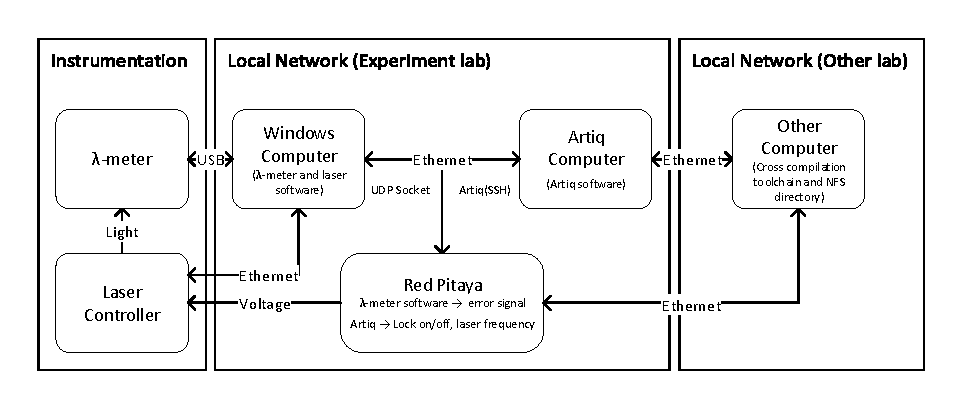
\includegraphics[width=\textwidth]{Images/schematic_before.pdf}
    \captionsetup{justification=centering}
    \caption{Laser frequency control instrumentation scheme at the beginning of the project.}
    \label{fig:schematic}
\end{figure}

For this project, the following objectives were set:
\begin{itemize}
\itemsep 0em % To reduce space between items
    \item To correct the fact that the cross compilation chain (oscimpDigital\footnote{oscimpDigital is an ecosystem designed to provide a consistent, chip independent, software/hardware cross-compile solution.} and Buildroot\footnote{Buildroot is a simple, efficient and easy-to-use tool to generate embedded Linux systems through cross-compilation.}) and the NFS directories were stored in \textit{Other laboratory's computer}, for which it was preferred to migrate them to the \textit{Artiq computer} (see section \ref{section:migration_section}).
    \item To have a standalone, single board computer running the Wavelength meter software and the C++ program, given that these two do not require a lot of computational power and that there are conflicts whenever a camera is connected via USB to the Windows Desktop computer (see section \ref{section:installation_windows10} and \ref{section:installation_lattepanda}).
    \item To fix the network communication software on the \textit{Red Pitaya} (written in C) and on the \textit{Windows computer} (written in C++), given that the communication between the two was not consistent, and it was necessary to close the socket twice whenever a new frequency setpoint was selected. Also, to implement a method that interrupts the communication process from the Artiq interface (see section \ref{subsec:udp_correction}).
    \item To have an automated start-up process to mount the NFS directory on the \textit{Red Pitaya} at power up, in case the latter had a power outage or just for a convenient everyday operation of the experiment (see section \ref{section:start_up_automation}).
\end{itemize}

\subsection{Migration of Red Pitaya environment between two computers}
\label{section:migration_section}

The migration process of the cross compilation chain (oscimpDigital and Buildroot) and the
NFS directory from the \textit{Other lab computer} to the \textit{Artiq computer} (as presented in figure \ref{fig:schematic}) is described in figure \ref{fig:migration_flowchart}.

\begin{figure}[!h]
    \centering
    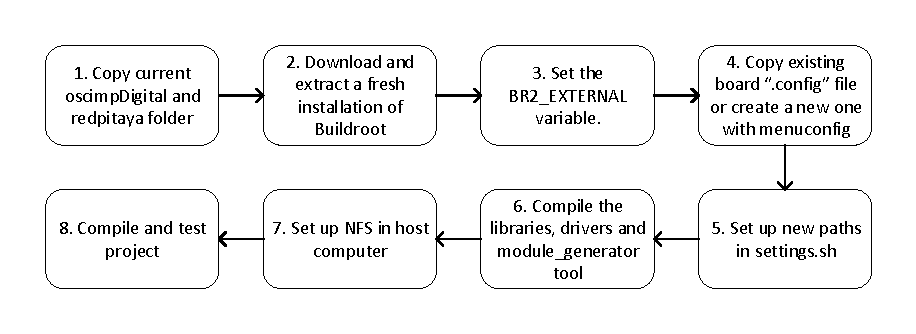
\includegraphics[width=0.95\textwidth]{Images/migration_flowchart.pdf}
    \captionsetup{justification=centering}
    \caption{Migration process flowchart.}
    \label{fig:migration_flowchart}
\end{figure}

%Step 1:
\begin{step}
The folders "oscimpDigital" and "redpitaya" were copied from the \textit{Other computer} to the \textit{Artiq computer} using the "scp" command (listing \ref{lst:copy_osc_red}).

\begin{lstlisting}[style=bash,label={lst:copy_osc_red},caption={Copying files from the \textit{Other computer} to the \textit{Artiq computer}.}]
cd /home/manip/redpitaya/
scp -r pyb@172.16.120.154:~/oscimp/oscimpDigital ./oscimpDigital_pyb
scp -r pyb@172.16.120.154:~/oscimp/redpitaya ./redpitaya_pyb
\end{lstlisting}

\end{step}

%Step 2:
\begin{step}
It was necessary to download and install Buildroot in the \textit{Artiq computer}, it's imperative to download the new Buildroot files before the compilation instead of using the existing ones from the \textit{Other computer}, the latter contain hard links that are not compatible with the new location.

Running "make" using the old files may lead to unwanted results, such as the usage of the entire hard-disk. First the version "2019.05-rc3" was downloaded from \hyperlink{https://buildroot.org/downloads/buildroot-2019.05-rc3.tar.gz}{https://buildroot.org/downloads/buildroot-2019.05-rc3.tar.gz} and then extracted (listing \ref{lst:unpack_buildroot}), the name of the resulting folder was changed from "buildroot-2019.05-rc3" to "buildroot-2019.05-rc3\_redpitaya\_pyb".

\begin{lstlisting}[style=bash,label={lst:unpack_buildroot},caption={Extracting Buildroot.}]
tar -xf buildroot-2019.05-rc3.tar.gz
rm buildroot-2019.05-rc3.tar.gz
\end{lstlisting}

\end{step}

%Step 3:
\begin{step}
As per trabucayre's "redpitaya" GitHub repository \cite{trabucayre}, we must set up the "BR2\_EXTERNAL" variable to the location where the "redpitaya" directory is, as show in listing \ref{lst:br2_external}, to provide Buildroot based support for Red Pitaya (12, 14, and 16 bits) board.

\begin{lstlisting}[style=bash,label={lst:br2_external},caption={Setting the BR2\_EXTERNAL variable.}]
export BR2_EXTERNAL=~/redpitaya/redpitaya_pyb/
\end{lstlisting}

\end{step}

%Step 4:
\begin{step}
In order to match the previous installation, the board configuration file (options and features selected for the resulting OS) was copied into the \textit{Artiq computer} and then compiled with the "make" command, the commands of listing \ref{lst:copy_config} were performed in the directory "/home/manip/redpitaya/buildroot-2019.05-rc3\_redpitaya\_pyb/".

\begin{lstlisting}[style=bash,label={lst:copy_config},caption={Copying board ".config" file to the new Buildroot directory.}]
scp pyb@172.16.120.154:~/oscimp/redpitaya_buildroot/.config ./
make
\end{lstlisting}

In the middle of the compilation, there was an error fetching the file "linux-xilinx-v2019.1.tar.gz" from the internet, which is why it was copied from the \textit{Other computer} directly (listing \ref{lst:linux-xilinx}).

\begin{lstlisting}[style=bash,label={lst:linux-xilinx},caption={Copying xilinx file from previous installation.}]
scp pyb@172.16.120.154:~/oscimp/redpitaya_buildroot/dl/linux/linux-xilinx-v2019.1.tar.gz ./linux/linux-xilinx-v2019.1.tar.gz
make
\end{lstlisting}

\end{step}

%Step 5:
\begin{step}
Once the cross-compilation toolchain was installed, the next step was to set up the NFS directory in the \textit{Artiq computer}, following the instructions of oscimp's GitHub repository "oscimpDigital" \cite{oscimp}, the designated location was "/home/manip/redpitaya/oscimpDigital\_pyb/nfs" (listing \ref{lst:mkdir_nfs}).

\begin{lstlisting}[style=bash,label={lst:mkdir_nfs},caption={Creating NFS directory.}]
mkdir /home/manip/redpitaya/oscimpDigital_pyb/nfs
\end{lstlisting}

Inside the directory "/home/manip/redpitaya/oscimpDigital\_pyb/" the "settings.sh" file was found, which contains all environment variable information required for the compilation of the library, drivers and modules, as shown in listing \ref{lst:nfs_settings}, only the "BR\_DIR" and "OSCIMP\_DIGITAL\_NFS" variables needed to be updated.

\begin{lstlisting}[style=bash,label={lst:nfs_settings},caption={Updating variables "settings.sh" file.}]
export BR_DIR='/home/manip/redpitaya/buildroot-2019.05-rc3_redpitaya_pyb'
export OSCIMP_DIGITAL_NFS='/home/manip/redpitaya/oscimpDigital_pyb/nfs'
\end{lstlisting}

\end{step}

%Step 6:
\begin{step}
The libraries (listing \ref{lst:libraries}), drivers (listing \ref{lst:drivers}) and modules (listing \ref{lst:modules}) must be compiled; however, for the latter, the Makefile fails at copying the file "module\_generator" to the "/usr/local/bin" directory, thus, this was done manually with the \textbf{sudo} command (listing \ref{lst:modules}, line 5).

\begin{lstlisting}[style=bash,label={lst:libraries},caption={Compiling the libraries.}]
cd /home/manip/redpitaya/oscimpDigital_pyb/lib
make install_ssh
\end{lstlisting}

\begin{lstlisting}[style=bash,label={lst:drivers},caption={Installing the drivers.}]
export PATH=~/redpitaya/buildroot-2019.05-rc3_redpitaya_pyb/output/host/usr/bin/:$PATH
cd /home/manip/redpitaya/oscimpDigital_pyb/linux_driver
make install_nfsdir
\end{lstlisting}

\begin{lstlisting}[style=bash,label={lst:modules},caption={Compiling the module generator tool.}]
cd /home/manip/redpitaya/oscimpDigital_pyb/app/tools/module_generator
chmod +x Makefile
make install

sudo cp module_generator /usr/local/bin
\end{lstlisting}

\end{step}

\begin{step}
To finish the configuration on the new host (\textit{Artiq computer}), the "nfs-kernel-server" must be installed and the rights of the nfs directory changed, which allowed to have access to bistreams, applications and drivers through the NFS shared directory, this is accomplished by running the commands in listing \ref{lst:nfs_kernel}. 

\begin{lstlisting}[style=bash,label={lst:nfs_kernel},caption={Installing nfs-kernel server and changing directory rigths.}]
apt install nfs-kernel-server nfs-common

cd /home/manip/redpitaya/oscimpDigital_pyb/nfs
chown -R $(id -u).$(id -g) .
\end{lstlisting}

\end{step}

\begin{step}
The last step of the migration process was to compile and test the project (UDP Client on Red Pitaya), for which the project files were copied from the \textit{Other computer} and then compiled (listing \ref{lst:compile_test_1}).

%Check if this is the correct location line 3 and 4
\begin{lstlisting}[style=bash,label={lst:compile_test_1},caption={Copying project files and compile.}]
cd ~/redpitaya/oscimpDigital_pyb/projects/
scp -r pyb@172.16.120.154:~/oscimp/projects ~/redpitaya/oscimpDigital_pyb/projects/
make && make install

cd ~/redpitaya/oscimpDigital_pyb/nfs/redpitaya/laser_lock_LSR/bin/
scp -r pyb@172.16.120.154:~/oscimp/nfs/redpitaya/laser_lock_LSR/bin/start_lock.sh ./
scp -r pyb@172.16.120.154:~/oscimp/nfs/redpitaya/laser_lock_LSR/bin/laser_lock_LSR_us.sh ./
\end{lstlisting}

Running the software gave a segmentation fault error, upon close examination, it was not able to create and access a file in the current directory due to missing rights (fixed in listing \ref{lst:compile_test_2} line 1), there was also a missing file on the project's bitstreams directory (fixed in listing \ref{lst:compile_test_2} line 3 to 4).

\begin{lstlisting}[style=bash,label={lst:compile_test_2},caption={Correcting directory rights and copying missing file on bitstreams.}]
chmod -R 777 ~/redpitaya/oscimpDigital_pyb/nfs/redpitaya

cd ~/redpitaya/oscimpDigital_pyb/projects/laser_lock_LSR/design
cp laser_lock_LSR_wrapper.bit.bin ~/redpitaya/oscimpDigital_pyb/nfs/redpitaya/laser_lock_LSR/bitstreams/
\end{lstlisting}

\textbf{Conclusion:} Finally, the Red Pitaya software was tested successfully and there is no longer a dependency on the \textit{Other computer}. The new instrumentation scheme, as shown in figure \ref{fig:schematic_2}, requires only two computers located in the experiment's laboratory.

\begin{figure}[!h]
    \centering
    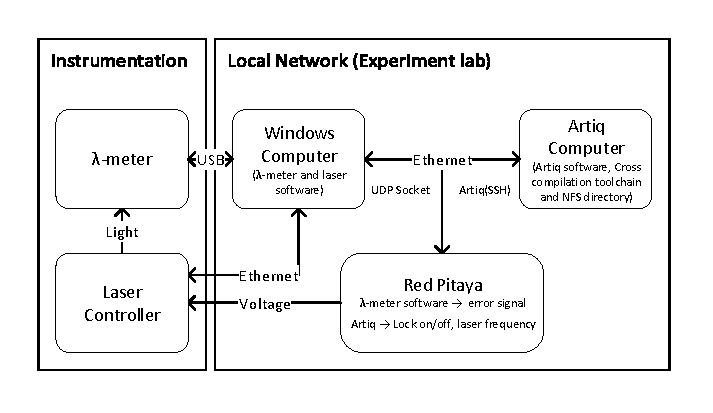
\includegraphics[width=0.8\textwidth]{Images/schematic_after_migration.pdf}
    \captionsetup{justification=centering}
    \caption{Laser frequency control instrumentation scheme after migration.}
    \label{fig:schematic_2}
\end{figure}

\end{step}

\subsection{Installation of Windows 10 on Raspberry Pi}
\label{section:installation_windows10}
%introduction: we had an issue because there are some error when we want to use the wavelength meter software together with a camera on windows computer#1. This is because of the wavelength meter (the manufacturer admitted it). We decided to move the wavelength meter to a minimalistic computer.
While trying to use simultaneously the wavelength meter and some USB camera, we had multiple crashes on the Windows computer. It turns out that the wavelength meter software is defective and is not compatible with the use of some cameras simultaneously. We decided to install the wavelength meter software on a different computer. In a first instance, the option to have the Wavelength meter software on a single board Raspberry Pi computer was explored, for which there were two options:

\begin{itemize}
\itemsep 0em % To reduce space between items
\item To install a precompiled Raspbian OS\footnote{OS: Operating System} and emulate a Windows environment (using Wine\footnote{Wine is a free and open-source compatibility layer that aims to allow application software and computer games developed for Microsoft Windows to run on Unix-like operating systems.}) in order to install and run the software. In case of success, to tailor an optimized Linux operating system with Buildroot.
\item To install a ARM Windows 10 OS.
\end{itemize}

\subsubsection{Installation of Raspbian OS and Wine32 on the Raspberry Pi}

One of the main challenges for this approach is the fact that the Raspberry Pi ARM-based processor is fundamentally different from the x86-based CPU found in a typical PC. It was necessary to install box86 to emulate a x86 system on the Raspberry Pi and then Wine 32 to run Windows applications. However, incompatibility issues were found.\\

Despite of the fact that it was possible to install the software with wine32, it was not possible to obtain a correct behavior from the GUI of the software, it presented black sections and it was unresponsive as show in figure \ref{fig:raspbian}. 

\begin{figure}[!h]
    \centering
    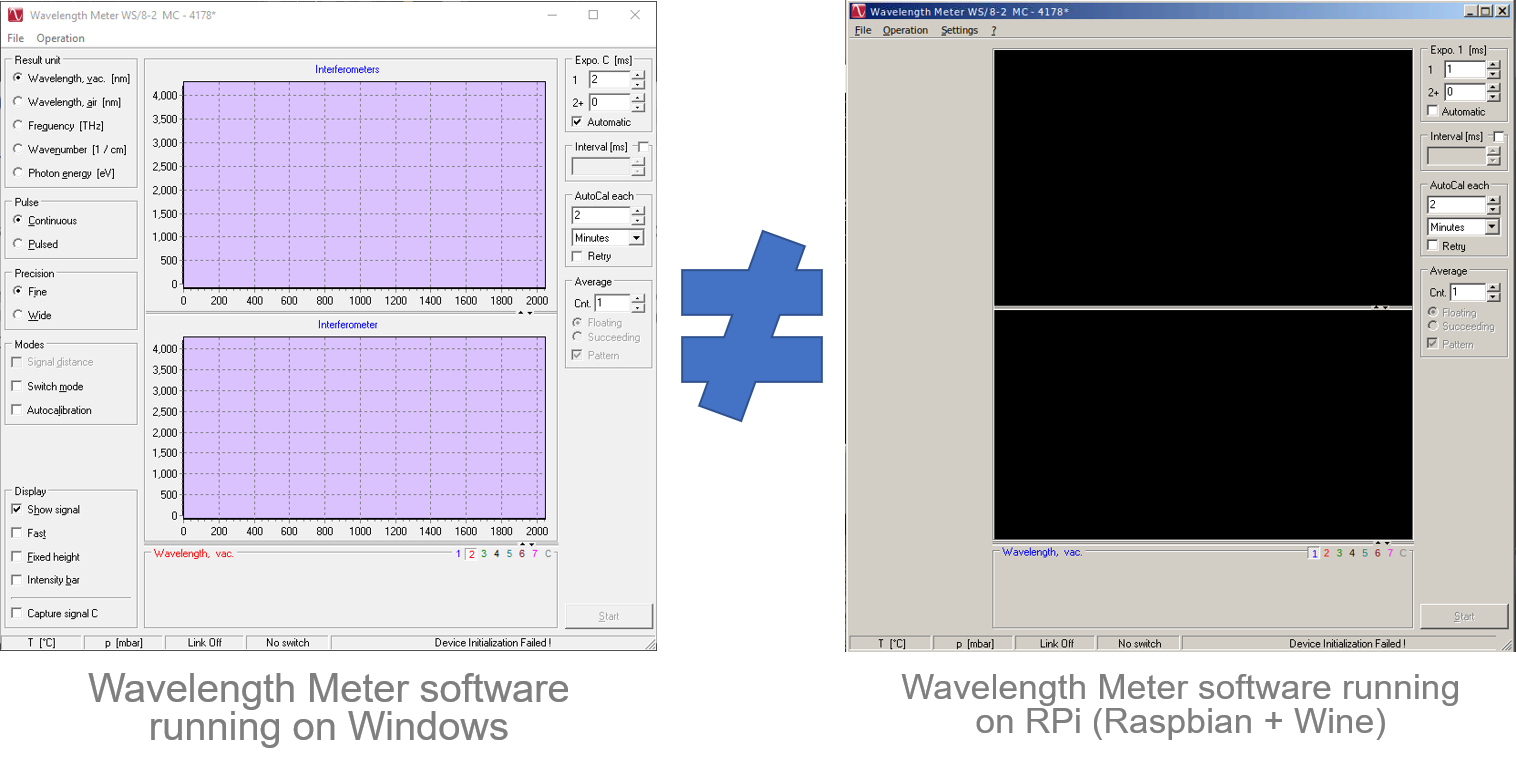
\includegraphics[width=0.8\textwidth]{Images/rapbian_results.png}
    \captionsetup{justification=centering}
    \caption{Results of installing the wavelength meter software on Raspbian.}
    \label{fig:raspbian}
\end{figure}

\subsubsection{Installation of ARM Windows 10 OS on the Raspberry Pi}

Since it was not possible to run the Wavelength meter software on Raspbian due to their architectures incompatibility, the next option was to install a Windows 10 ARM version, which is compatible with the Raspberry Pi 4 and allows to run native Windows applications, it developed by the WoR (Windows on Raspberry Pi) project.

There is no legal way to download ISO files for Windows 10 ARM. Instead, a legal UUP dump file was downloaded, or "Unified Update Platform". This is a way for Microsoft to share its latest advances within its "Insider Preview" program. In short, the process was to download the UUP file, build a full ISO image from that file on the computer, then flash that ISO to boot on the Raspberry Pi.

With this approach it was possible to install the software on the Raspberry Pi. However, at initialization the device was not found (figure \ref{fig:device_not_found}), even though at installation a driver was installed. This appears to be an issue with the operating system which doesn't provide yet full support for peripherals such as USB ports. 

\begin{figure}[!h]
    \centering
    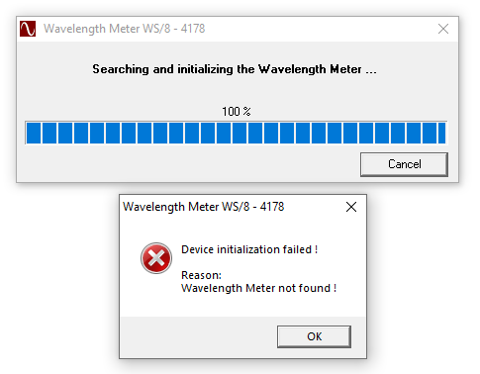
\includegraphics[width=0.4\textwidth]{Images/device_not_found.png}
    \captionsetup{justification=centering}
    \caption{ARM Windows on RPi error: Wavelenth Meter not found.}
    \label{fig:device_not_found}
\end{figure}

\textbf{Conclusion:} The Raspberry Pi with ARM Windows was not robust enough to accommodate the software and be reliable in a daily basis operation, due to its slow speed and being prone to freeze or reset.

\subsection{Installation of Wavelength meter on Latte Panda single board computer}
\label{section:installation_lattepanda}

Finally, it was decided to install the Wavelength meter software on a Latte Panda single board computer (figure \ref{fig:latte_panda}) with the specifications described in table \ref{table:latte_panda_specs}.

\renewcommand{\arraystretch}{1.1}

\begin{table}[!h]
\begin{tabular}{ | l | l | }
\hline
\textbf{Processor}          & Intel Cherry Trail Z8350 Quad Core, 2M Cache, up to 1.92 GHz  \\ \hline
\textbf{Operating system}   & Pre-installed Windows 10                                      \\ \hline
\textbf{Ram}                & 4GB DDR3L                                                     \\ \hline
\textbf{Storage Capability} & 64GB                                                          \\ \hline
\textbf{GPU}                & Intel HD Graphics, 12 EUs @200-500 Mhz, single-channel memory \\ \hline
\textbf{Connectivity}       & WiFi and Bluetooth 4.0                                        \\ \hline
\textbf{Peripherals}        & One USB 3.0 port and two USB 2.0 ports                         \\ \hline
\textbf{Dimension of board} & 88 mm * 70 mm                                                    \\ \hline
\end{tabular}
\caption{Specifications of LattePanda 4G/64G.}
\label{table:latte_panda_specs}
\end{table}

\begin{figure}[!h]
    \centering
    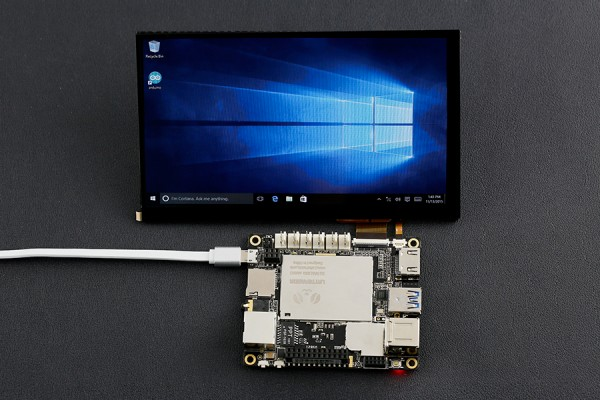
\includegraphics[width=0.4\textwidth]{Images/LattePanda.jpg}
    \captionsetup{justification=centering}
    \caption{LattePanda single board computer running a full version of Windows 10.}
    \label{fig:latte_panda}
\end{figure}


\textbf{Conclusion:} The installation was flawless for both the Wavelength meter software as well as the UDP Server. After testing, it was possible to establish a connection from the LattePanda UDP Server to the Red Pitaya UDP Client, thus control the laser frequency from the Artiq interface. The resulting instrumentation scheme is presented in figure \ref{fig:schematic_3}.
%old: when the UDP socket must be closed by the Red Pitaya (see section \ref{subsec:udp_correction})

%Add screenshots/photos of the software working on the LattePanda.
% \textcolor{red}{Photos pending}

\begin{figure}[!h]
    \centering
    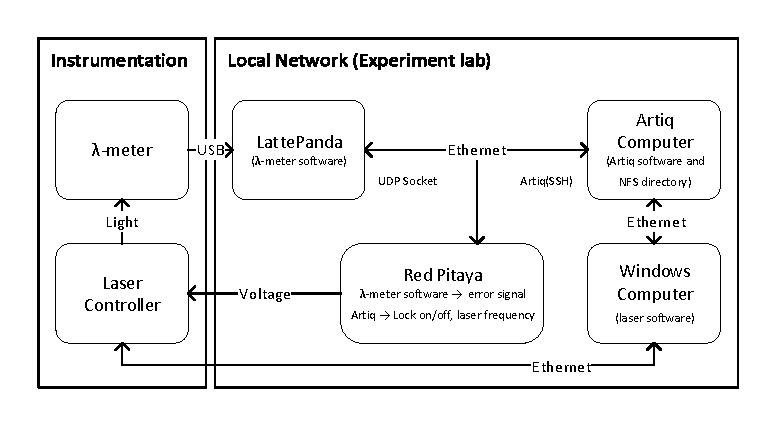
\includegraphics[width=0.8\textwidth]{Images/schematic_final_stage.pdf}
    \captionsetup{justification=centering}
    \caption{Laser frequency control instrumentation scheme after the addition of LattePanda.}
    \label{fig:schematic_3}
\end{figure}

\newpage
\subsection{Correction of network communication between Red Pitaya and Wavelength meter}
\label{subsec:udp_correction}

The frequency measured by the wavelength meter is sent to the \textit{Red Pitaya} so that it can generate an error signal. Since the wavelength meter software comes with C++ libraries, it was chosen to use a UDP protocol to exchange information between the \textit{Windows computer} (running the wavelength meter software) and the \textit{Red Pitaya}.

An UDP datagram-based protocol was implemented before I started the internship. However this process was erratic and required the client socket (Red Pitaya) to be closed twice every time a new setpoint was selected. To circumvent this problem, a series of scripts were created and run from the \textit{Artiq computer} (SSH control of the Red Pitaya) but it was intended to have a robust and reliable network communication for the experiment that would also allow future enhancements to the instrumentation scheme.

\textit{Normally in the UDP protocol, the client does not form a connection with the server like in TCP and instead just sends a datagram to request for data. Similarly, the server doesn't need to accept a connection and just waits for datagrams request to arrive} \cite{geeksforgeeks_2022}, as show in figure \ref{fig:server-and-client}. However, upon closer inspection of the server and client code, the flowchart of figure \ref{fig:udp_before} was deduced.

\begin{figure}[!h]
    \centering
    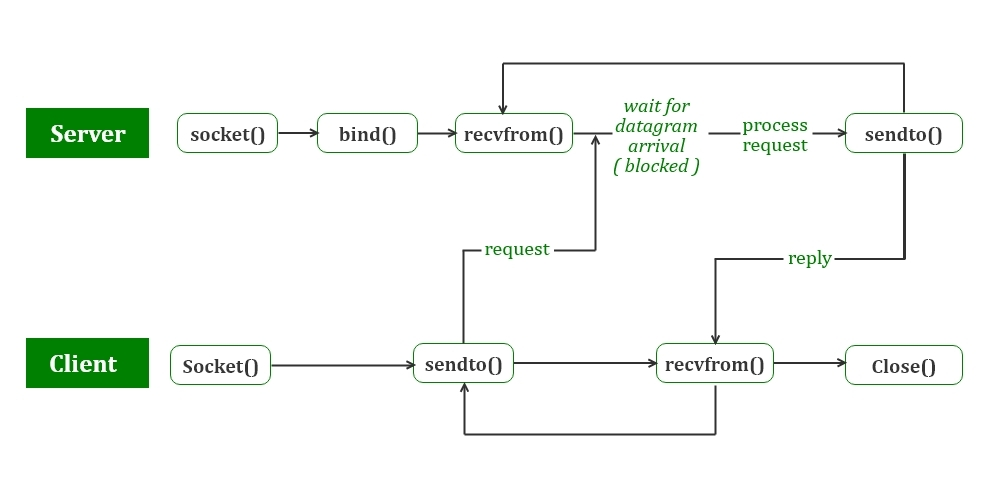
\includegraphics[width=0.8\textwidth]{Images/server-and-client.jpg}
    \captionsetup{justification=centering}
    \caption{Standard UDP protocol \cite{geeksforgeeks_2022}}
    \label{fig:server-and-client}
\end{figure}

\begin{figure}[!h]
    \centering
    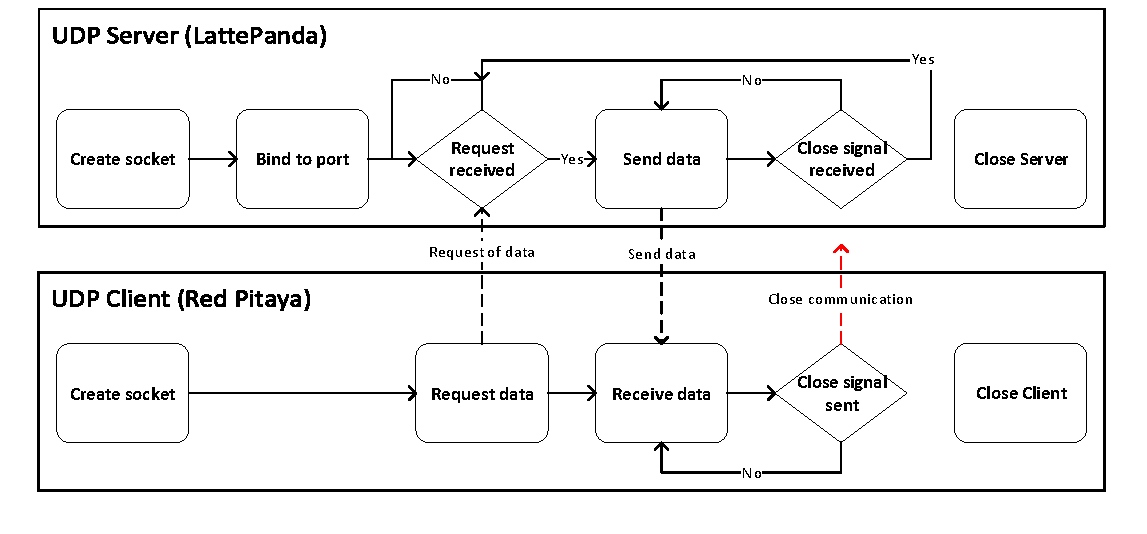
\includegraphics[width=0.9\textwidth]{Images/UDP_before.pdf}
    \captionsetup{justification=centering}
    \caption{Implemented UDP protocol before improvements.}
    \label{fig:udp_before}
\end{figure}

\newpage
There was a miscommunication between the Client and the Server, in which the former was not able to send the "close signal" in order to terminate the process (i.e to establish a new setpoint and start again). The solution implemented is shown in figure \ref{fig:udp_after}.

\begin{figure}[!h]
    \centering
    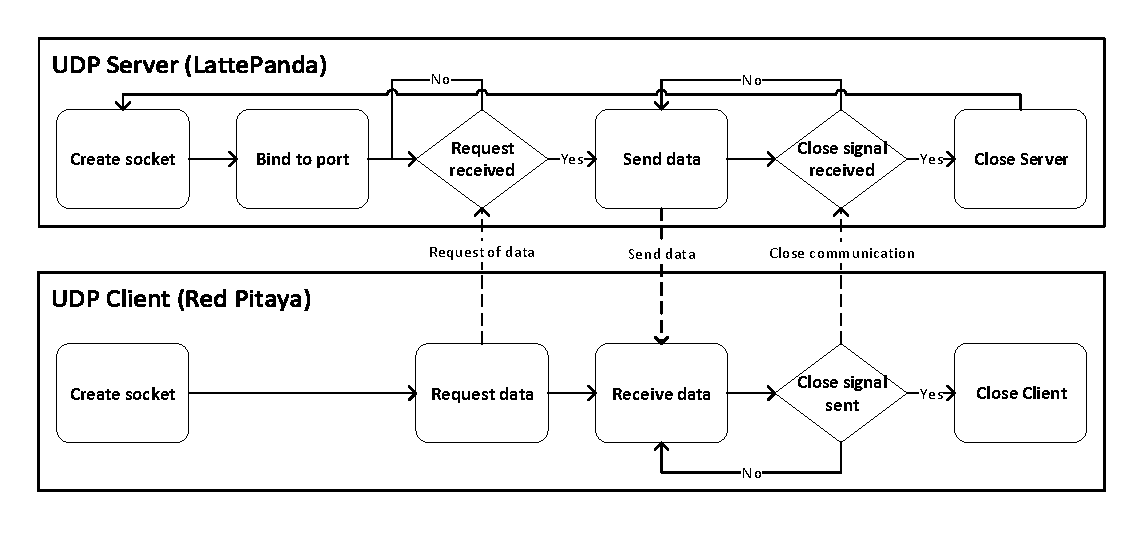
\includegraphics[width=0.9\textwidth]{Images/UDP_after.pdf}
    \captionsetup{justification=centering}
    \caption{Implemented UDP protocol after improvements.}
    \label{fig:udp_after}
\end{figure}

First for the Server code (listing \ref{lst:server_close}), a "while" loop was introduced (line 101) to ensure that every time a "close signal" is received, the socket is closed and a new one is created and bound to the port. Thus, every time the Server sends information to the Client, it also verifies if the latter has replied back with the word "Bye" (line 227 to 230), if that is the case, the code "breaks" out of the first loop (line 229) and then out of the main loop (line 235), effectively restarting the process by closing the socket (line 237) and continuing from the start again (line 106).

\pagebreak
\lstinputlisting[nolol=true,label={lst:server_close},caption={Key elements of the improved Server code (not complete code).},style=c++,widthgobble=1*3,linerange={101-101,106-109,116-127,142-150,153-157,171-171,184-184,196-197,220-220,227-231,234-242}]{Code/windows software.cpp} \vspace{0.4cm}

Then for the Client, as exhibited in listings \ref{lst:client_close} and  \ref{lst:client_close2}, the method used to close the socket in real time (and avoid interrupting the data exchange that locks the laser frequency), was to have a file named "stop\_pid" in the Red Pitaya, which by default contains a "0" (line 181 to 189), that is read after every cycle of the main "while" loop (line 285 to 293). When the content of the file is set to "1" by the Artiq program, the socket is closed and the "while" loop quits (line 291 and 292 respectively). 
\lstinputlisting[nolol=true,label={lst:client_close},caption={Client code, creation of "stop\_pid" file.},style=c++,widthgobble=1*3,linerange={181-189}]{Code/laser_lock_LSR.c} \vspace{0.4cm}

\lstinputlisting[nolol=true,label={lst:client_close2},caption={Client code, checking the "stop\_pid" file to close the socket.},style=c++,widthgobble=2*3,linerange={285-293}]{Code/laser_lock_LSR.c} \vspace{0.4cm}

As previously mentioned and presented in figure \ref{fig:udp_before}, the Client must send a "close signal" to the Server in order to restart the socket, this is performed inside the "close\_udp()" function, as shown in listing \ref{lst:close_udp}, the word "Bye" is sent using the "sendto" (line 111) function and then the Client socket itself is closed (line 112).

\lstinputlisting[nolol=true,label={lst:close_udp},caption={Client side "close\_udp" function.},style=c++,widthgobble=0*3,linerange={108-113}]{Code/laser_lock_LSR.c} \vspace{0.4cm}

% \subsection{Improvement of UDP socket closing method} %This section is explained in the previous one.

\subsection{Automation of NFS mounting and program execution at startup of Red Pitaya}
\label{section:start_up_automation}

In order to automate the NFS directory mounting and the program execution at startup, multiple approaches were considered and tested. However, the most reliable was do add a bash script in the system directory "/etc/network/if-up.d/", all the scripts stored there are executed once the network connection is established.

\pagebreak
\begin{lstlisting}[style=bash,label={lst:startup},caption={Automated NFS mounting and program execution script.}]
#!/bin/sh

echo ">>Mounting /opt/" > /dev/kmsg
sleep 5
mount /opt/

node_process_id=$(pidof laser_lock_LSR_us)
if [[ -z $node_process_id ]]; then
echo "$SERVICE stopped"
echo ">>Running laser lock" > /dev/kmsg
cd /opt/redpitaya/laser_lock_LSR/bin
./laser_lock_LSR_us.sh
./start_lock.sh &
fi
\end{lstlisting}

The implemented bash script is shown in listing \ref{lst:startup}, first the "\/opt" directory is mounted after a 5 seconds delay (line 3 to 5), then the "laser lock" program is executed in case it was not running (line 7 to 14). It's worth pointing out that the ampersand symbol added to the execution of the program in line 13 is critical, given that the program must run in the background.

\subsection{Partial conclusion}

After these improvements, the laser frequency lock for the blue laser is more robust, hands-free, and the wavelength meter can be operated from the \textit{LattePanda} without affecting the cameras of the experiment.

%% Second project
\newpage
\section{Improvements on CPT-based Cs microcell Atomic Clock pedagogical model}
\subsection{Introduction}
\label{section:tp_info}
The atomic clock described in this section is used in the yearly European Frequency and Time Seminar (EFTS) hosted at ENSMM\footnote{ENSMM: École Nationale Supérieure de Mécanique et des Microtechniques.}, \textit{which is a no-profit intensive full-week seminar intended to provide education and training with lectures and lab sessions to a broad audience: Engineers, Ph.D. students, post-docs, young scientists, newcomers, etc. }\cite{efts}

The following section has been extracted from the practical work document \cite{tp}. Figure \ref{fig:globalcpt} shows the architecture of a miniature Cs cell atomic clock based on coherent population trapping (CPT).

\begin{figure}[h!]
	\centering
	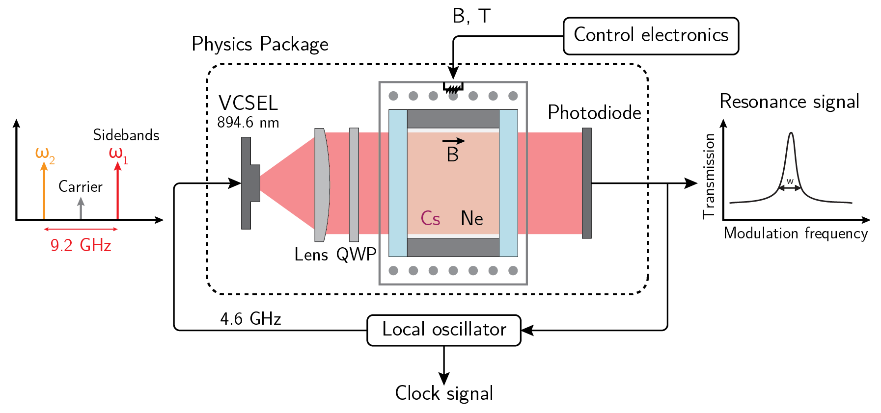
\includegraphics[width=0.9\linewidth]{Images/globalCPT.png}
	\caption{Simplified architecture of a buffer-gas filled Cs microcell CPT atomic clock.}
	\label{fig:globalcpt}
\end{figure}

Cs vapor is filled in a glass-silicon-glass micro-fabricated cell whose technology is described in~\cite{hasegawa}. The Cs cell is filled with a pressure buffer gas. The buffer gas slows down atoms in the microcell and increases the time for the atoms to reach the cell walls. It also reduces the first-order Doppler effect and leads to operation in the Lamb-Dicke regime~\cite{dicke}. Eventually, it helps to detect narrow CPT resonances.

Atoms in the cell interact with a dual-frequency (in the ideal case) optical field generated by a VCSEL laser whose injection current is directly modulated at 4.596 GHz through a bias-tee. This generates two first-order optical sidebands separated by about 9.192 GHz, required to produce the CPT interaction. The laser output beam crosses a neutral density filter to attenuate the optical power and a quarter-wave plate to polarize circularly the optical beam. The light transmitted through the cell is detected by a photodiode.

When the frequency difference between both first-order optical sidebands exactly equals the Cs ground-state hyperfine splitting (9.192 631 770 GHz), atoms are trapped through a quantum interference process in a quantum superposition of both ground states (see Fig.~\ref{fig:ppeCPT}). In this so-called dark state, the light atomic absorption is reduced and the atomic vapor transparency is increased. The CPT resonance linewidth is ultimately limited by the microwave CPT coherence relaxation time and can be measured to be of about 1 kHz in a buffer-gas filled micro-fabricated cell. The signal at the output of the photodiode is used in two main servo loops. The first one is dedicated to the stabilization of the laser frequency onto the bottom of a homogeneously broadened optical line. The second loop stabilizes the local oscillator (LO) frequency onto the atomic clock transition.

\begin{figure}[h!]
	\centering
	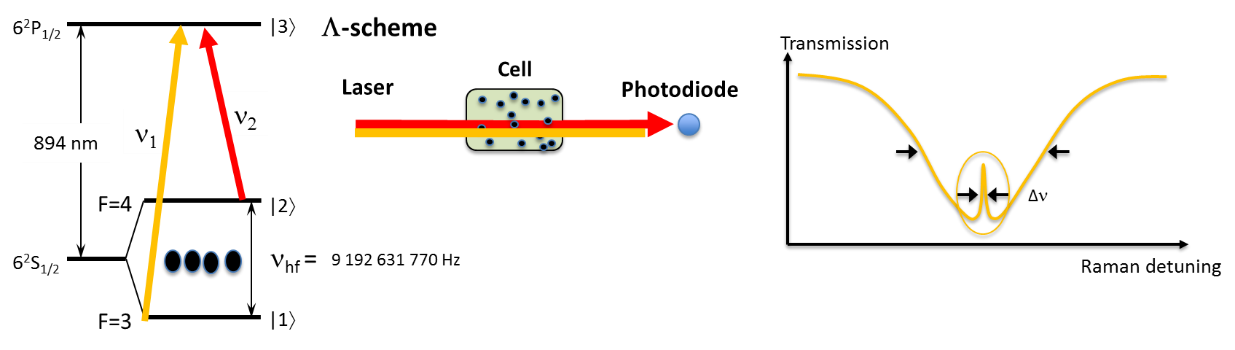
\includegraphics[width=0.8\linewidth]{Images/ppeCPT.png}
	\caption{Basic principle of CPT.}
	\label{fig:ppeCPT}
\end{figure}

\newpage
\subsubsection{Laser servo loop}

% \newsavebox{\laserAnimation}
% \sbox{\laserAnimation}{\animategraphics[width=0.5\textwidth,autoplay,loop]{2}{animation_laser_servo_loop/laser1_}{0}{36}}

% \newsavebox{\quartzAnimation}
% \sbox{\quartzAnimation}{\animategraphics[controls={play,step},width=0.5\textwidth,autoplay,loop]{2}{animation_quartz_servo_loop/quartz_}{0}{61}}

The purpose of the laser servo loop is to set and lock the laser current (i.e. laser frequency) in the bottom of the absorption profile where the CPT signal is located. As shown in figure \ref{fig:laser_servo_loop}, the laser current is shift to the right and left by a fixed modulation width and the photodiode measurements are recorded in two variables ("val1" and "val2"). The error signal is then calculated as the difference between "val1" and "val2".

\begin{figure}[!h]
\centering
\begin{subfigure}[c]{0.49\textwidth}
	\centering
	\animategraphics[controls={play,step},width=\textwidth,autoplay,loop]{2}{animation_laser_servo_loop/laser1_}{0}{50}
	\captionsetup{justification=centering}
\end{subfigure}
\hfill
\begin{subfigure}[c]{0.49\textwidth}
	\centering
	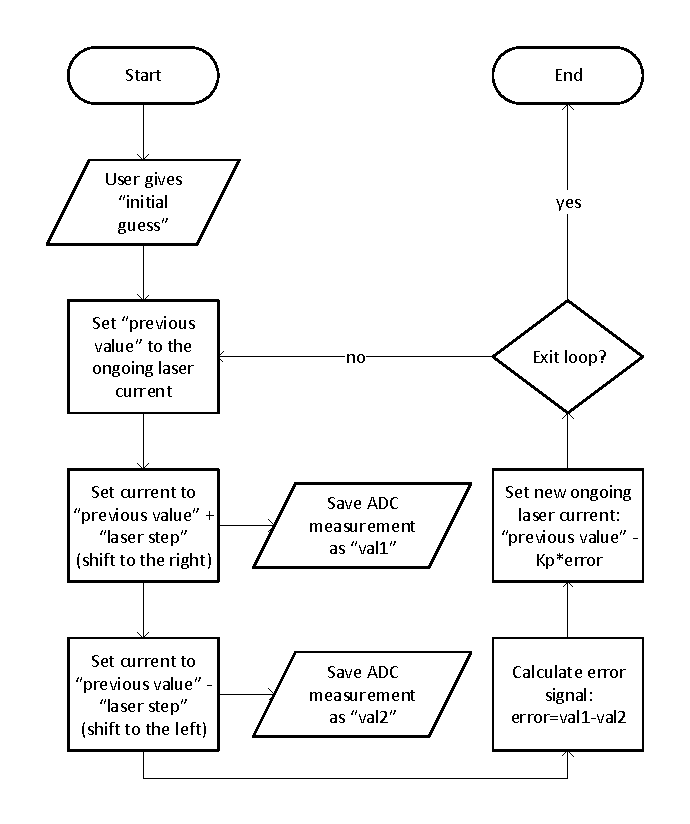
\includegraphics[width=\textwidth]{Images/Laser_Servo_loop_flowchart.pdf}
	\captionsetup{justification=centering}
\end{subfigure}
 \caption{Laser servo loop.}
\label{fig:laser_servo_loop}
\end{figure}

The calculated error signal can be used to adjust the laser current to an equilibrium point between the two modulation values ("val1" and "val2"). To determine the new laser current, the error signal is multiplied by a gain "Kp" and the process is repeated until the user decides to stop the servo loop. 

By adjusting the values of the modulation width and the gain "Kp", it is possible to obtain a fast response with a deterioration in the stability of the loop, or vice-versa, a slow and steady response.

\subsubsection{Quartz servo loop}

Similar to the laser servo loop, the quartz servo loop relies on setting an initial frequency and then modulate it to calculate an error signal (we want the error signal to be equal to 0). As shown in figure \ref{fig:quartz_servo_loop}, the process to lock the quartz frequency is to first set the initial PLL frequency by applying a voltage to the VCO\footnote{VCO: Voltage Controlled Oscillator.} of the 10 Mhz quartz oscillator (which is the reference for the PLL). Next, using the PLL synthesizer and its frequency-shift keying capability (when the logical value of pin 12 "TXDATA" changes), the central carrier frequency of the PLL is shifted by 1 kHz to the right in the frequency domain (i.e. the frequency is increased by 1 kHz).

The photodiode measurements before and after the modulation are recorded and are used to calculate the error signals. These error signals are used with a PID controller to lock the PLL frequency to an equilibrium point.

\begin{figure}[!h]
\centering
\begin{subfigure}[c]{0.49\textwidth}
	\centering
	\animategraphics[controls={play,step},width=\textwidth,autoplay,loop]{2}{animation_quartz_servo_loop/quartz_}{0}{61}
	\captionsetup{justification=centering}
\end{subfigure}
\hfill
\begin{subfigure}[c]{0.49\textwidth}
	\centering
	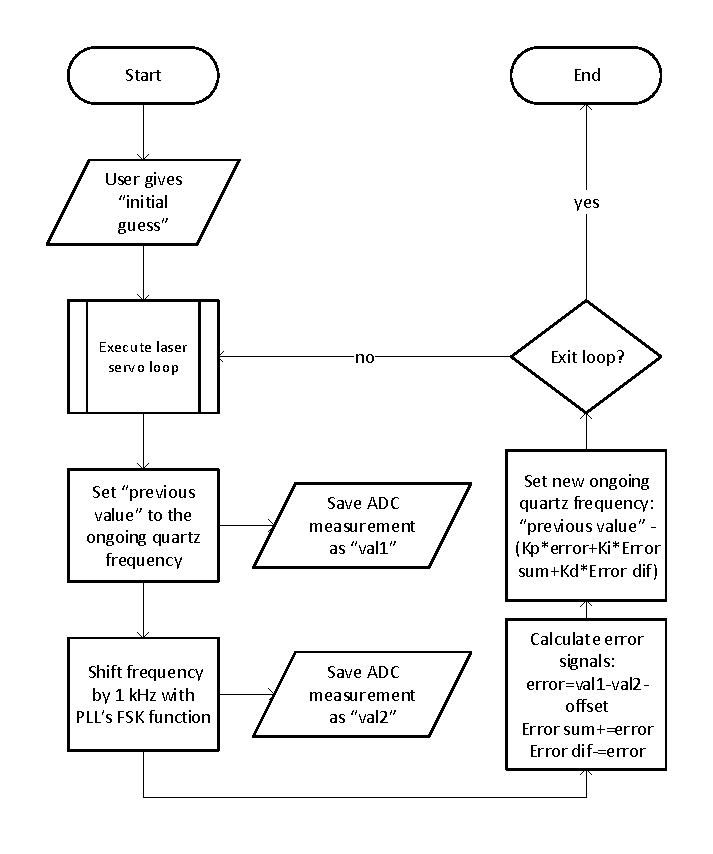
\includegraphics[width=\textwidth]{Images/Quartz_Servo_loop_flowchart.pdf}
	\captionsetup{justification=centering}
\end{subfigure}
 \caption{Quartz servo loop.}
\label{fig:quartz_servo_loop}
\end{figure}

The reason why the equilibrium point is found around half of the transmission peak height and not at its maximum value, is due to the fact that the values compared are the ongoing PLL frequency and the 1 kHz right shifted PLL frequency. When both frequencies produce the same output in the photodiode, the error signal is 0 and the locked frequency is found at the ongoing PLL frequency, i.e. to the left of the transmission peak, this is demonstrated in figure \ref{fig:transmission_peak}.

\begin{figure}[h!]
	\centering
	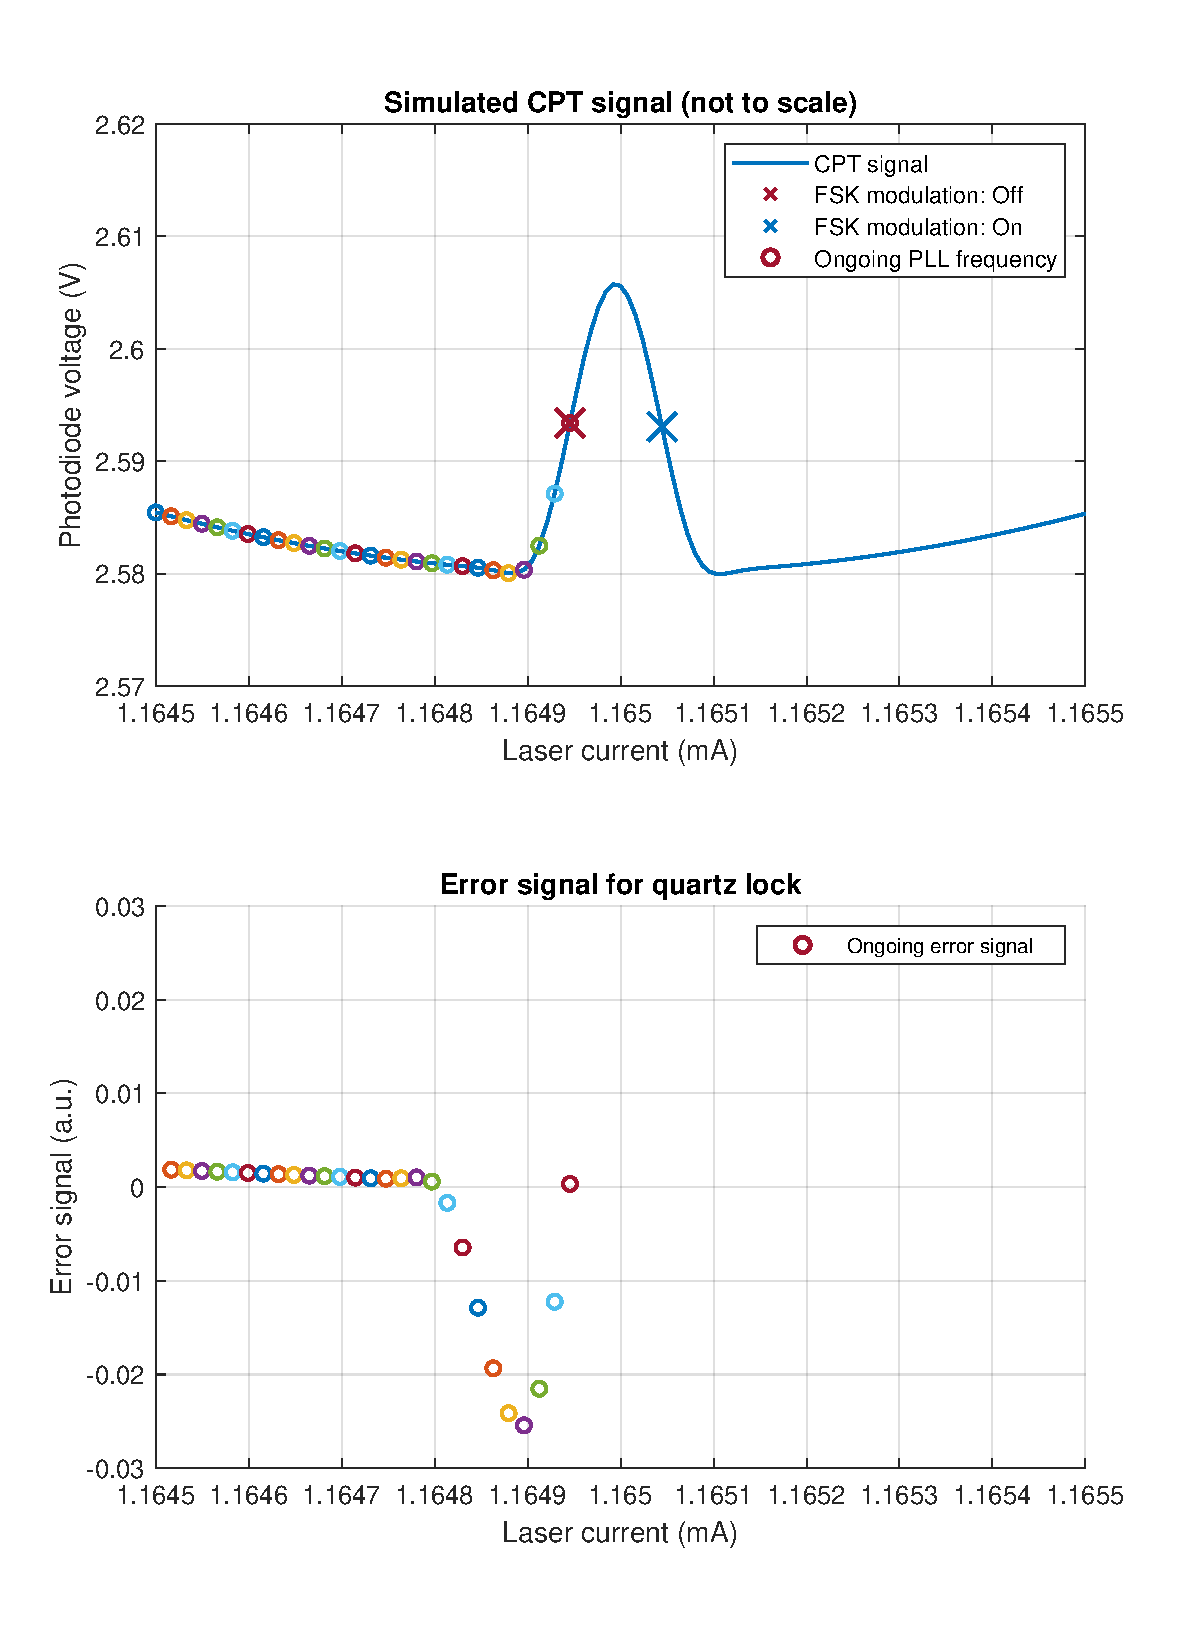
\includegraphics[width=0.5\textwidth]{animation_quartz_servo_loop/quartz_28.pdf}
	\caption{Locked frequency at half of the transmission peak height.}
	\label{fig:transmission_peak}
\end{figure}

% \vfill
\newpage
\subsection{Context}
When I started my contribution to this project, there were three atomic clocks, out of which only one was working perfectly (hereafter referred to as \textit{Clock 1}). The other two were marginally operational, with a weak absorption signal and low signal-to-noise ratio. This made it very difficult to lock the servo loops on the desired electronic transition. Moreover, the GUI\footnote{GUI: Graphical User Interface, is a series of visual components that allow the interaction between the user and the program.} used (see figure \ref{fig:gui_v1.6}) was not intuitive.

The project had plenty of room for improvement, due to  the following reasons:

\begin{itemize}
\itemsep 0em % To reduce space between items
    %Controls
    \item The control of the demonstrator relied on non-intuitive commands typed in the software's console, for example, typing \texttt{"t 30000 s"} to generate a ramp that started from the laser current equal to "30000" \textit{machine units}\footnote{Machine units, are positive integer values from 0 to $2^{16}$ that are used by the code but have no evident relation with real physical units.}, (see section \ref{section:replacement_serial}).
    \item All the units used in the program were \textit{machine units} instead of real physical units such as volts, amperes and Hertz. This was very counterproductive pedagogically speaking, (see section \ref{section:physical_units}).
    \item A panel named "Control" was present but some of their elements were not operational (e.g. laser temperature control) and others were not relevant for the operation of the demonstrator (such as the Synthesizer control elements, since the synthesizer is controlled internally for every function), (see section \ref{section:replacement_serial}).
    \item It was not possible to change the quartz oscillator scan parameters (initial and final scan values), (see section \ref{section:scan_params}).
    %Main operation
    \item It was necessary to press a physical button outside the demonstrator to stop a never-ending loop process, i.e "Laser scan" or "Laser lock", (see section \ref{section:stop_process}).
    \item An oscilloscope had to be connected at all times to the demonstrator in order to monitor the output of the photodiode, (see section \ref{section:output_monitoring}).
    %Graphical
    \item The graphs were missing titles and axis labels, (see section \ref{section:graphs}).
    \item Since the demonstrator worked only with \textit{machine units} and with the oscilloscope measurements, it was difficult to identify the laser current value for maximum absorption, (see section \ref{section:max_absorb}).
    \item It was difficult to identify when the servo loops got locked or unlocked.
    % \item It was not intuitive when the servo loops were locked, only the time plots were available. %Covered in previous item
    \item When doing a quartz scan\slash modulation, it was only possible to visualize the "error signal" but not the CPT signal itself, (see section \ref{section:CPT}).
    %Others
    
\end{itemize}

\begin{figure}[!h]
    \centering
    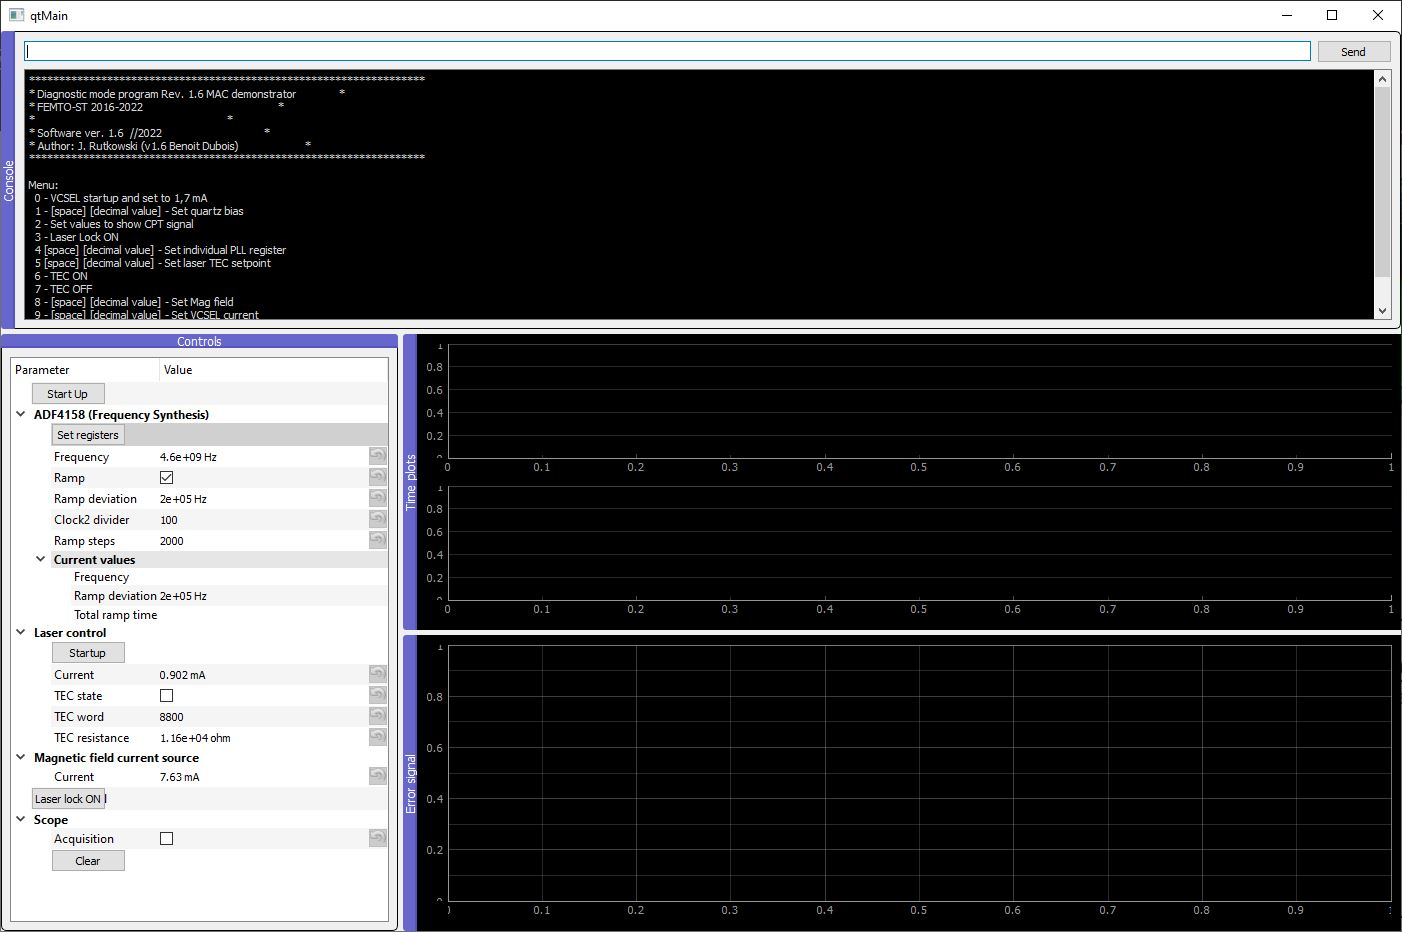
\includegraphics[width=\textwidth]{Images/GUI_v1.6.JPG}
    \captionsetup{justification=centering}
    \caption{Micro Atomic Clock demonstrator program before improvements, version 1.6.} 
    \label{fig:gui_v1.6}
\end{figure}

While working on this project I was able to modify both the Python based GUI and the Arduino based microcontroller code to overcome these problems, in order to have a more reliable, intuitive, easy to use and robust atomic clock demonstrator. Furthermore, I fixed two of the non-operational atomic clocks (see section \ref{section:repair_atomic_clocks}).

The improvements added in the context of this year's EFTS, were well received and appreciated by my supervisors and the participants to the seminar, to the point of being honored by the event's chair, Dr. Enrico Rubiola, with a recognition diploma for my contribution.
\pagebreak

\subsection{Physical components}

\begin{figure}[!h]
    \centering
    \includegraphics[width=0.8\textwidth]{Images/mac.png}
    \captionsetup{justification=centering}
    \caption{Components of the atomic clock demonstrator.} 
    \label{fig:mac_components}
\end{figure}

The atomic clock demonstrator (see figure \ref{fig:mac_components}) consist of the following components:

\begin{enumerate}[wide, labelwidth=!, labelindent=0pt]
	\item \textbf{AC power connector.}
	\item \textbf{Power supply: } Converts the 240 VAC from mains voltage to 12 VDC.
	\item \textbf{Voltage regulator: } Steps down the 12 VDC coming from the power supply to 5 V and 3.3 V. 
	\item \textbf{Arduino Due and shield connector: } Main processing unit to control of the system, its content can be programmed with the same USB port used to operate the clock; the shield provides a connector for the "Atomic clock board".
	\item \textbf{Physical package: } This includes the VCSEL, photodiode (with a current to voltage circuit), heating element for the vapor cell and the coil to provide a static magnetic field. The terminals allow a convenient way to unmount it from the main board. The coaxial RF jack, connects to a Bias-Tee that mixes the laser current with the microwave signal coming from the synthesizer.
    \item \textbf{Cell temperature controller: } This circuit contains an Atmega 32u4 microcontroller to implement a PID controller, a power stage to drive the heating element and an ADC to measure the temperature and close the control loop. The program of the best working clock (\textit{Clock 1}) was extracted and flashed on the \textit{Clock 2 and 3} (listing \ref{lst:flash}).
    
    \begin{lstlisting}[style=bash,label={lst:flash},caption={Read operation to extract microcontroller's binary (Windows CMD).}]
C:\Users\cmrivera\AppData\Local\Arduino15\packages\arduino\tools\avrdude\6.3.0-arduino17/bin/avrdude -CC:\Users\cmrivera\AppData\Local\Arduino15\packages\arduino\tools\avrdude\6.3.0-arduino17/etc/avrdude.conf -v -patmega32u4 -cavr109 -b57600  -PCOM18 -D -Uflash:r:readfile.hex:i
    \end{lstlisting}
    
    \begin{lstlisting}[style=bash,label={lst:flash},caption={Write operation to flash microcontroller's binary (Windows CMD).}]
C:\Users\cmrivera\AppData\Local\Arduino15\packages\arduino\tools\avrdude\6.3.0-arduino17/bin/avrdude -CC:\Users\cmrivera\AppData\Local\Arduino15\packages\arduino\tools\avrdude\6.3.0-arduino17/etc/avrdude.conf -v -patmega32u4 -cavr109 -PCOM18 -b57600 -D -Uflash:w:C:\Users\cmrivera\Desktop\readfile.hex:i 
    \end{lstlisting}
    
    \item \textbf{Connector of external laser temperature controller.}
    \item \textbf{ADC circuit:} In charge of converting the photodiode signal to digital units for the microcontroller. Its resolution can be programmed (see section \ref{section:output_monitoring}).
    \item \textbf{Photodiode signal: } This RF coaxial coupling is connected to the oscilloscope to monitor the photodiode signal.
    \item \textbf{Frequency synthesizer: } Generates the microwave signal necessary to have CPT resonance (see section \ref{section:tp_info}), it consists of a fractional-N frequency synthesizer (ADF4158) connected to a voltage-controlled oscillator (V950ME21-LF) through a loop filter (schematic in figure \ref{fig:sch_synth}). It also provides the modulation to find the error signal for the quartz servo loop, by using FSK (Frequency-shift keying). 
    \item \textbf{Microwave signal attenuator:} In order to control the amount of microwave power mixed with the laser signal, in the practical work, attendees are asked to turn the signal off and then gradually increase it.
    \item \textbf{RF splitter:} To measure the microwave signal.
    \item \textbf{Microwave signal connector: } To monitor the microwave signal on a spectrum analyzer.
    \item \textbf{Component to ensure the microwave signal doesn't reflect into the system.}
    \item \textbf{Physical button:} To interrupt scan or lock processes ran by the microcontroller.
    \item \textbf{USB connector.}
\end{enumerate}

\newpage
\subsection{Improvement of Graphical User Interface and Arduino code}

\subsubsection{Replacement of serial commands by visual control elements}
\label{section:replacement_serial}

To avoid the use of arbitrary and non-intuitive commands on the program's "Console" panel, the complete "Controls" panel was redesigned (as shown in figure \ref{fig:new_gui}), allowing to type in the desired values in labeled boxes and start\slash stop processes with buttons, while the "console commands" were generated and sent to the microcontroller in the background. 

\begingroup
\setlength{\intextsep}{0pt}%
\setlength{\columnsep}{10pt}%
\begin{wrapfigure}{L}{0.4\textwidth}
    % \vspace{-10pt}
    \centering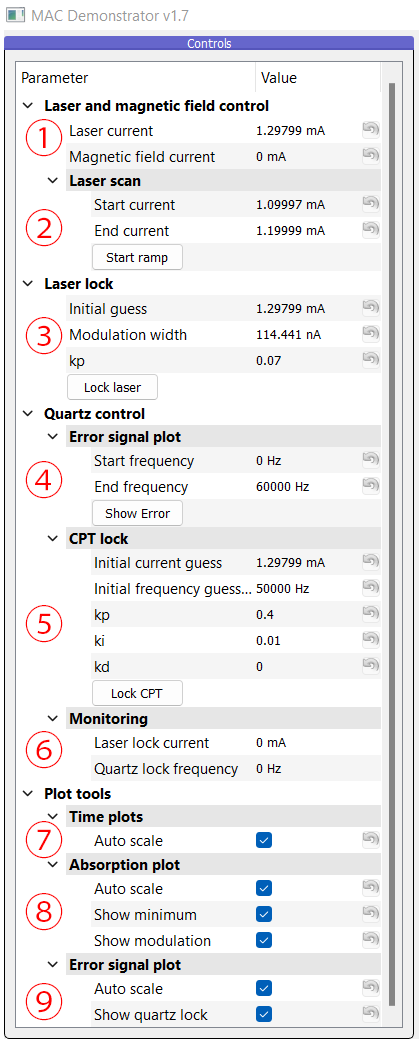
\includegraphics[width=\linewidth, left]{Images/controls.png}
    \captionsetup{justification=centering}
    \caption{New control panel.}
    \label{fig:new_gui}
\end{wrapfigure}

The description of each control's function will be progressively explained in this report, since they correspond to a specific feature added. Nonetheless, from figure \ref{fig:new_gui} we may identify the following groups:

\begin{enumerate}[wide, labelwidth=!, labelindent=0pt]
	\item \textbf{Laser and magnetic field control:} \newline These two controls were already present in the previous GUI and rely on the console commands \texttt{"9 \{laser current\}"} and  \texttt{"8 \{magnetic field current\}"}, to modify the laser current DAC\footnote{DAC: Digital-to-Analog Converter, is a system that converts a digital signal into an analog signal.} and magnetic field current DAC respectively. %When their value is changed, the commands are replaced with their content and sent to the microcontroller.
	
	\item \textbf{Laser and magnetic field control | Laser scan:} \newline Previously, it was only possible to set the start of the laser ramp with command \mbox{\texttt{"t \{start\}"}}, however this function was modified to also take \mbox{\texttt{"t \{start\} \{end\} \{number of samples\}"}} \break(the \texttt{"number of samples"} was set to 300 by default).
	
	The console command \texttt{"s"}, used to start the ramp process, is now linked with the button "Start ramp".
	\item \textbf{Laser lock:} \newline To lock the laser frequency, it was only possible to select an "initial guess", with the command \mbox{\texttt{"i \{initial guess\}"}}. In order to set the current in the vicinity of the desired absorption. However, the modulation width was fixed at 38.147nA (1 in \textit{machine units}).\newline Now it is also possible to select a modulation width, the graphical controls are linked with the command \mbox{\texttt{"i \{initial guess\} \{modulation width\}"}}. This greatly enhances the locking capability by giving more flexibility to the user, and solved the fact it was difficult to lock with the old program's version. %Explain how the laser lock works so this makes sense.
	\newline The "Lock laser" button is linked with the previous command \texttt{"l"}.
 	\item \textbf{Quartz control | Error signal plot:} \newline In the old version of the program, the command \texttt{"b"} allowed to scan the quartz frequency \textbf{only} from 0 to 41530 (\textit{machine units}) or from 0 to 67.486 kHz. This was improved, and now it is possible to set the "start" and "end" scan frequencies (see section \ref{section:scan_params}).
 	\newline The button "Show Error" is linked with the previous command \texttt{"b"}.
\end{enumerate}
\endgroup

\begin{enumerate}[wide, labelwidth=!, labelindent=0pt]
    \setcounter{enumi}{4} % To set the first number
    \item \textbf{Quartz control | CPT lock:} \newline Formerly, the CPT locking process (locking both servo loops simultaneously) used the commands \mbox{\texttt{"a \{quartz kp\} \{quartz ki\} \{quartz kd\} \{laser kp\}"}} to set the PID parameters and \texttt{"0"} to start. But it was impossible to change the "initial guess" for the frequency offset, this value was hard-coded to be 16.25 kHz.
    \vfill
    After my modifications, it is possible to set an arbitrary "initial guess" frequency and PID parameters from the GUI's entry boxes (see section \ref{section:scan_params}).
    \newline The button "Lock CPT" is linked with the previous command \texttt{"0"}.
    \item \textbf{Quartz control | Monitoring:} \newline This panel of read-only labels was added to have the real-time locking values of the laser and quartz servo loops, and thus, avoid relying on the graphs and graphical estimation.
	\item \textbf{Plot tools | Time plots:} \newline An option to enable or disable auto-scale from the plots was added. 
	\item \textbf{Plot tools | Absorption plot:} \newline  Two visual aid tools were implemented for the absorption profile graph: A minimum value marker (see section \ref{section:max_absorb}) and a pair of lock modulation markers (see section \ref{section:lock/unlock}).

	\item \textbf{Plot tools | Error signal plot:} \newline A lock offset frequency marker was added for both the "Error signal" and "CPT signal" plots. Which allow monitoring in real time the locking status of the demonstrator (see section \ref{section:lock/unlock}).
	
% 	\begin{figure}[!h]
%     \centering
%     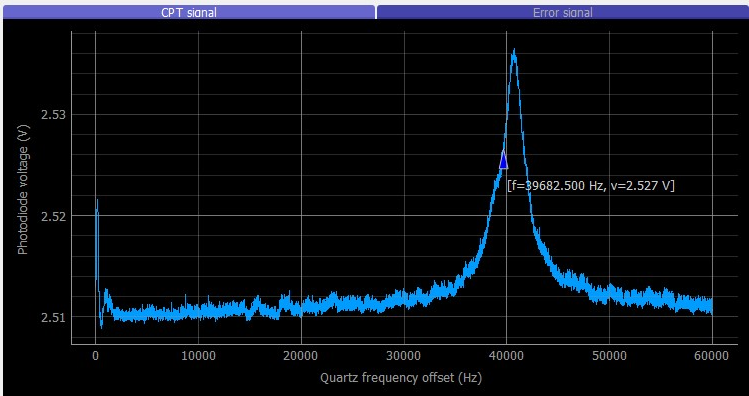
\includegraphics[width=0.6\textwidth]{Images/plot_tools_2.png}
%     \captionsetup{justification=centering}
%     \caption{Plot tools for the CPT and Error signal} 
%     \label{fig:plot_tools_2}
%     \end{figure}
\end{enumerate}

\subsubsection{Conversion from machine units to physical units}
\label{section:physical_units}

One of the main shortcomings the project presented at the beginning of my internship, was the fact that both the commands to control the demonstrator, and the graphs of the GUI were in \textit{machine units}. Since these were the values that the microcontroller handled with the ADC and DAC and no conversion mechanism was implemented yet.

This lead to a non-intuitive experience for the seminar attendees, that were not able to work with real physical units and thus, not fully conceptualize the theoretical information received. 

The solution was to determine a linear relation between the machine and physical units. First, by carrying-out measurements that later were used to fit a curve with the correct coefficients needed to create conversion functions for both the microcontroller and the Python GUI.
\subsubsubsection{Machine units to photodiode voltage and vice-versa}
\label{section:word_to_volt}
In order to create a conversion function, it was necessary to determine the correct coefficients for a linear fit. To do this, five arbitrary laser current values were set, and the photodiode output was measured both with the demonstrator's ADC and with a connected oscilloscope. The results are shown in figure \ref{fig:word_to_volt}, as expected a linear relation can be extracted.

\begin{figure}[!h]
    \centering
    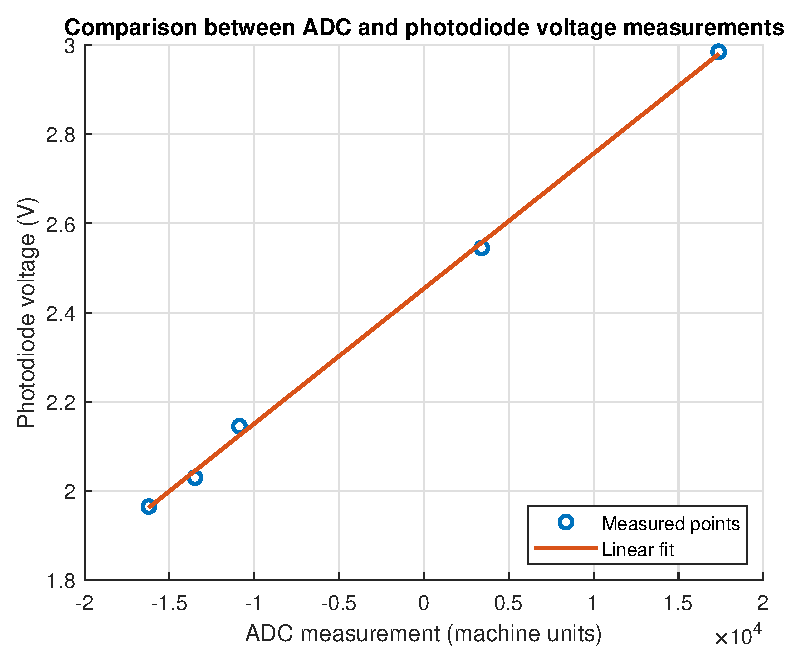
\includegraphics[width=0.6\textwidth]{Images/word_to_voltage.eps}
    \captionsetup{justification=centering}
    \caption{Comparison between ADC and photodiode voltage measurements.} 
    \label{fig:word_to_volt}
\end{figure}

The linear fit was computed with MATLAB (file: Conversion\_Functions\_Coefficients.m) and the coefficients in equation \ref{eq:word_to_volt_1} were found, and the expressions at equation \ref{eq:word_to_volt_2} deduced.
\begin{align}
y=p1*x+p2\quad
\begin{cases}
p1=\SI{3.0295e-05}{}\\ p2=2.4539
\end{cases}
\label{eq:word_to_volt_1}
\\voltage=p1*ADC+p2 \quad\text{and}\quad ADC=\frac{(voltage-p2)}{p1}
\label{eq:word_to_volt_2}
\end{align}

To verify the conversion factor, an arbitrary point in the absorption profile was selected and the measurements between the GUI and oscilloscope were compared. As shown in figure \ref{fig:word_to_volt_ver}, the values are close enough. 
As per equation \ref{eq:word_to_volt_2}, the implemented conversion functions are presented in listing \ref{lst:word_to_volt}.

\begin{figure}[!h]
\centering
\begin{subfigure}[b]{0.85\textwidth}
	\centering
	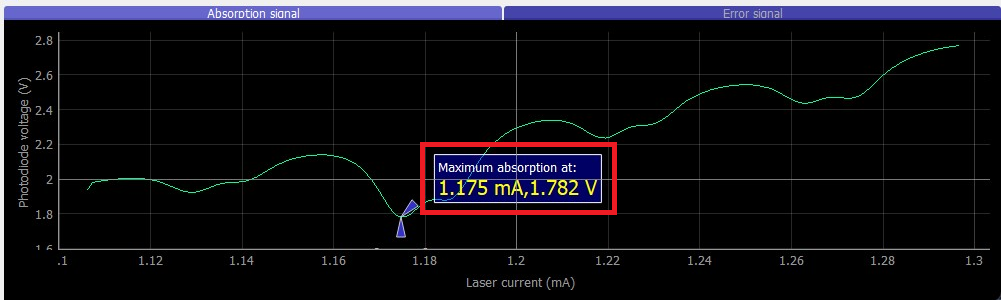
\includegraphics[width=\textwidth]{Images/word_to_volt_ver_1.png}
	\captionsetup{justification=centering}
\end{subfigure}
\newline
\begin{subfigure}[b]{0.85\textwidth}
	\centering
	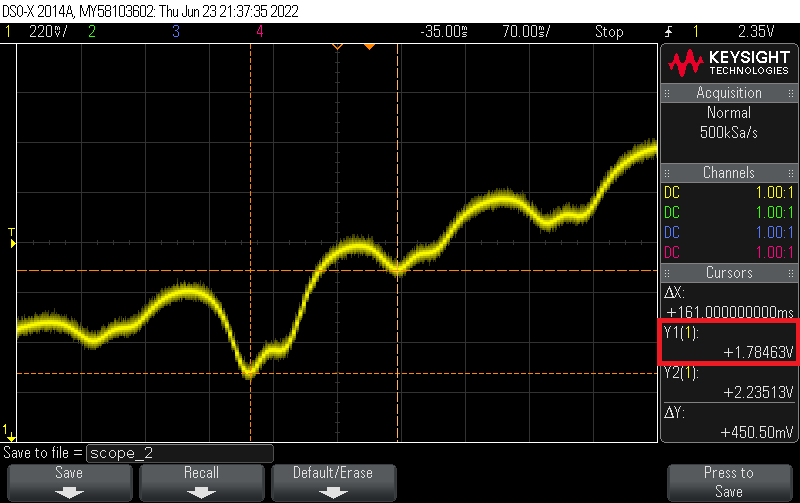
\includegraphics[width=\textwidth]{Images/word_to_volt_ver_2.png}
	\captionsetup{justification=centering}
\end{subfigure}
 \caption{Conversion factor verification for the word to voltage function.}
\label{fig:word_to_volt_ver}
\end{figure}

\begin{lstlisting}[style=python,label={lst:word_to_volt},caption={Python functions to convert machine units to voltage (file: misc.py).},firstnumber=151,escapeinside={\%}{\%}]
def word_to_voltage(value): %\addtocounter{lstnumber}{1}%
    p1=0.000030294604198194861416565740186435
    p2=2.4538899853718616483888581569772 %\addtocounter{lstnumber}{4}%
    return p1*value+p2

def voltage_to_word(value): %\addtocounter{lstnumber}{1}%
    p1=0.000030294604198194861416565740186435
    p2=2.4538899853718616483888581569772 %\addtocounter{lstnumber}{4}%
    return int((value-p2)/p1)
\end{lstlisting}
\subsubsubsection{Machine units to frequency offset and vice-versa}

Similar to the previous section (see \ref{section:word_to_volt}), we wish to determine the correct coefficients and linear relation between the set values for the quartz's DAC and the frequency shift (measured with a spectrum analyzer). To do this, 14 measurements were performed, and plotted in figure \ref{fig:word_to_freq}.

\begin{figure}[!h]
    \centering
    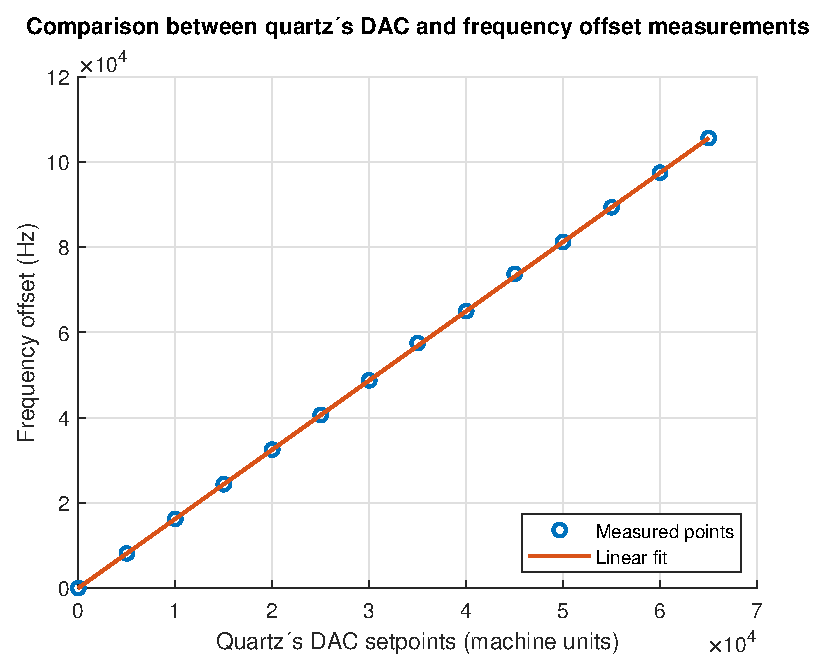
\includegraphics[width=0.6\textwidth]{Images/word_to_frequency.eps}
    \captionsetup{justification=centering}
    \caption{Comparison between quartz's DAC and frequency offset measurements.} 
    \label{fig:word_to_freq}
\end{figure}

Since only the frequency offset is required, the coefficient "$p2$" is disregarded. The resulting equations (equation \ref{eq:word_to_freq_1} and \ref{eq:word_to_freq_2}) were implemented in python, as shown in listing \ref{lst:word_to_frequency}.
\begin{align}
y=p1*x+p2\quad
\begin{cases}
p1=1.6250\\ p2=\SI{7.4299e-12}{} \approx 0
\end{cases}
\label{eq:word_to_freq_1}
\\frequency=p1*DAC \quad\text{and}\quad DAC=\frac{frequency}{p1}
\label{eq:word_to_freq_2}
\end{align}
\begin{lstlisting}[style=python,label={lst:word_to_frequency},caption={Python functions to convert machine units to frequency offset (file: misc.py).},firstnumber=171]
def word_to_frequency(value):
    p1=1.625
    p2=0
    return p1*value+p2

def frequency_to_word(value):
    p1=1.625
    p2=0
    return int((value-p2)/p1)
\end{lstlisting}

\subsubsubsection{Machine units to laser current and vice-versa}
\label{section:word_to_current}
The function to convert laser current to machine units was already present in the code. In listing \ref{lst:word_to_current}, the python class "LaserCurrentSource" contains a "setter decorator" method (line 49) that converts the input value (in mA) to machine units (line 52) and sends the appropriate command (line 53).

\begin{lstlisting}[style=python,label={lst:word_to_current},caption={Python function to convert laser current to machine units (file: mac\_device.py).},firstnumber=49]
@current.setter
def current(self, value):
    assert 0 <= value < 1.7
    self._current_word = int((value/2.5)*2.**16)
    self.parent.send("9 " + str(self._current_word))
\end{lstlisting}

\subsubsubsection{Machine units to magnetic field current and vice-versa}
Just as in the previous section (\ref{section:word_to_current}), the function to convert magnetic field current to machine units was present in the code as part of a "setter decorator" method, as shown in listing \ref{lst:word_to_mag}.

\begin{lstlisting}[style=python,label={lst:word_to_mag},caption={Python function to convert magnetic field current to machine units (file: mac\_device.py).},firstnumber=65]
@current.setter
def current(self, value):
    assert 0 <= value < 50
    self._current_word = int(value / 50. * (2.**16))
    logging.debug(self._current_word)
    self.parent.send("8 " + str(self._current_word))
\end{lstlisting}

% \subsubsection{Modification of Control panel elements}
% \label{section:control_elements}

\subsubsection{Flexibility to choose quartz oscillator scan and lock parameters}
\label{section:scan_params}

Due to the limitations of the previous quartz functions, two new commands have been added to the microcontroller code. First, the "start" and "end" frequencies for the quartz scan are no longer hard-coded, and it's possible to change them with the command \mbox{\texttt{"v \{start\} \{end\}"}} (listing \ref{lst:v_command}).

\begin{lstlisting}[style=c++,label={lst:v_command},caption={Command to change the quartz's scan parameters (file: mac.ino).},firstnumber=483]
//case 'v':
void QuartzScanSetStart(){
  scanQuartzStart=Serial.parseInt();
  scanQuartzEnd=Serial.parseInt();  
}
\end{lstlisting}

And lastly, the "initial guess" and "offset" for the quartz lock frequency can be changed with the command \mbox{\texttt{"j \{initial guess\} \{offset\}"}} (listing \ref{lst:j_command}).

\begin{lstlisting}[style=c++,label={lst:j_command},caption={Command to change the quartz's lock "initial guess" frequency (file: mac.ino).},firstnumber=472]
//case 'j':
void setQuartzLockParameters(){
  quartz_init = Serial.parseFloat();
  quartz_offset = Serial.parseFloat();
}
\end{lstlisting}

Both commands are linked with their respective graphical control elements.

\subsubsection{Interruption of processes through GUI}
\label{section:stop_process}

In the old version of the demonstrator program (version 1.6), it was necessary to press a physical button (mounted on the external housing) in order to interrupt a scan or lock process. This was not practical and introduced vibrations to the system. This is why a GUI solution was convenient.

Every button in the GUI has a double function, for example as shown in listing \ref{lst:button_function}, when the "Lock CPT" button is pressed, the lock process starts (line 662) and its name changes to "Unlock CPT" (line 661). Thus, next time the button is pressed, since its name is no longer "Lock CPT" (condition of line 660), the "else" statement of line 664 to 665 is executed.

\begin{lstlisting}[style=python,label={lst:button_function},caption={Double function for GUI buttons (file: qt\_mac.py).},firstnumber=659]
def action_start_CPT_lock(self):
    if("Lock CPT" == self.btn_start_CPT_lock.name()):
        self.btn_start_CPT_lock.setName("Unlock CPT")
        self.mac.lock_cpt()
    else:
        self.btn_start_CPT_lock.setName("Lock CPT")
        self.mac.stop_signal()
\end{lstlisting}

The "stop\_signal()" method sends the character "x" to the demonstrator microcontroller (listing \ref{lst:stop_signal}).

\begin{lstlisting}[style=python,label={lst:stop_signal},caption={Stop signal method (file: mac\_device.py).},firstnumber=245]
def stop_signal(self):
    self.send("x")
\end{lstlisting}

Previously, the only way to stop a process was by pressing the external physical button (e.g. in the laser lock function, listing \ref{lst:stop_methods}, line 515). Now there is also a condition, checked at every iteration, that if the character "x" is received from the GUI, the loop must be exited (line 516 to 520).

\begin{lstlisting}[style=c++,label={lst:stop_methods},caption={Stop signal methods in laser lock function (file: mac.ino).},firstnumber=515]
while(ButtonState == LOW){
    if(Serial.available()){
        if((char)Serial.read()=='x'){
            break;
        }
    }
\end{lstlisting}

\subsubsection{Photodiode output monitoring independent of oscilloscope}
\label{section:output_monitoring}

Originally, the demonstrator could only be used by relying on an oscilloscope connected to the photodiode output, this defeated the purpose of having a compact, all contained device. This is why it was decided to add a graph with the photodiode signal (through an ADC), as presented in figure \ref{fig:absorption_graph}.

\begin{figure}[!h]
    \centering
    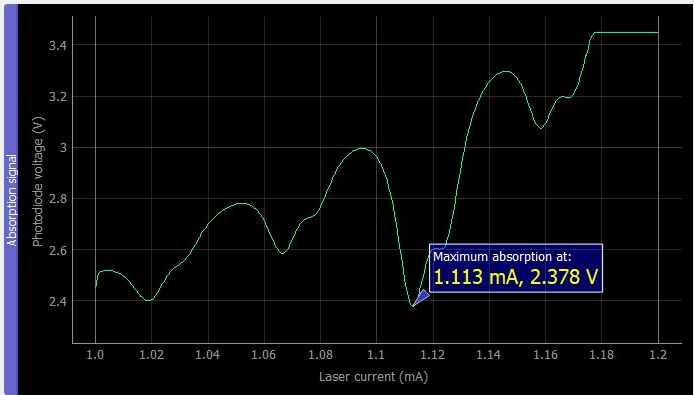
\includegraphics[width=0.5\textwidth]{Images/absorption_signal.png}
    \captionsetup{justification=centering}
    \caption{"Absorption signal" plot feature.} 
    \label{fig:absorption_graph}
\end{figure}

In the practical work, students are asked to estimate the threshold current of the VCSEL\footnote{VCSEL: Vertical-cavity surface-emitting laser, is a type of semiconductor laser diode with laser beam emission perpendicular from the top surface.} laser of the demonstrator. The threshold current of a laser is the current value at which the laser output power stops being 0 V and becomes linear, in other words, the value at which the laser emission can begin.

To find the threshold current of the laser, a scan from 0 to 1.7 mA (the maximum current used in the demonstrator) must be performed. However, a limitation was found. The ADC was able to measure only a fraction of the signal, as shown between the oscilloscope cursors in figure \ref{fig:adc_limitation}, the applied ramp went from 0 to 5 V, but the ADC measured only the values between 1.46 and 3.4 V approximately.
%picture
\begin{figure}[!h]
\centering
\begin{subfigure}[b]{0.49\textwidth}
	\centering
	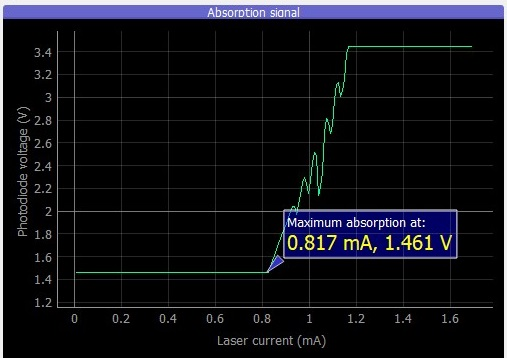
\includegraphics[height=0.6\textwidth]{Images/fsr_screenshot.jpg}
	\captionsetup{justification=centering}
\end{subfigure}
\hfill
\begin{subfigure}[b]{0.49\textwidth}
	\centering
	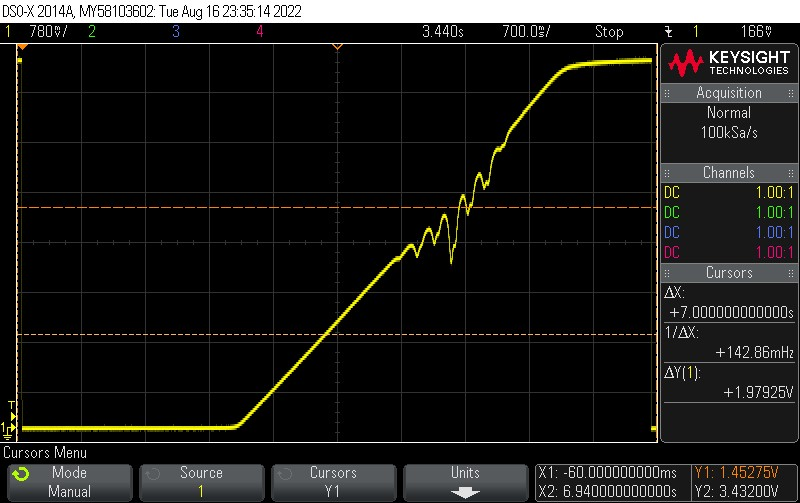
\includegraphics[height=0.6\textwidth]{Images/fsr_oscilloscope.jpg}
	\captionsetup{justification=centering}
\end{subfigure}
 \caption{Demonstrator's ADC limitation found.}
\label{fig:adc_limitation}
\end{figure}

Due to this limitation, it is imperative to use the oscilloscope, at least for the first part of the practical work. After analyzing the microcontroller code, it was found the ADC initialization function (listing \ref{lst:ADC_init}). The bits sent over SPI communication indicated that the FSR\footnote{FSR: Full-Scale Range of the ADC scaling that relies on the internal programmable gain amplifier (PGA).} was set to \mbox{1.024 V} (according to the ADC ADS1118 datasheet).
%listing
\begin{lstlisting}[style=c++,label={lst:ADC_init},caption={ADC\_startup() function (file: mac.ino).},firstnumber=421,literate={mu}{$\mu$}1]
void ADC_startup() { // Starts ADS1118, FSR = 1.024 V
  SPI.setDataMode(SPI_MODE1);
  digitalWrite(CS_ADC, LOW);
  SPI.transfer(B00000110); // CR: ADC FSR = 1.024V, since Ref is 2.5 V, 
  SPI.transfer(B11100011); // CR: the measurement range is from 1.4760 V to 3.5240 V
  digitalWrite(CS_ADC, HIGH); // CR: with a LSB size of 31.25 muV (LSB = FSR / 2^16).
  SPI.setDataMode(SPI_MODE0);
}
\end{lstlisting}

Upon analysis of the ADC schematic (figure \ref{fig:adc_sch}) it was found that the reference value of the ADC is 2.5 V (ADM7150 voltage regulator). Thus, the full measure range of the ADC was determined in equation \ref{eq:full_range_1}.
%schematic
\begin{figure}[!h]
    \centering
    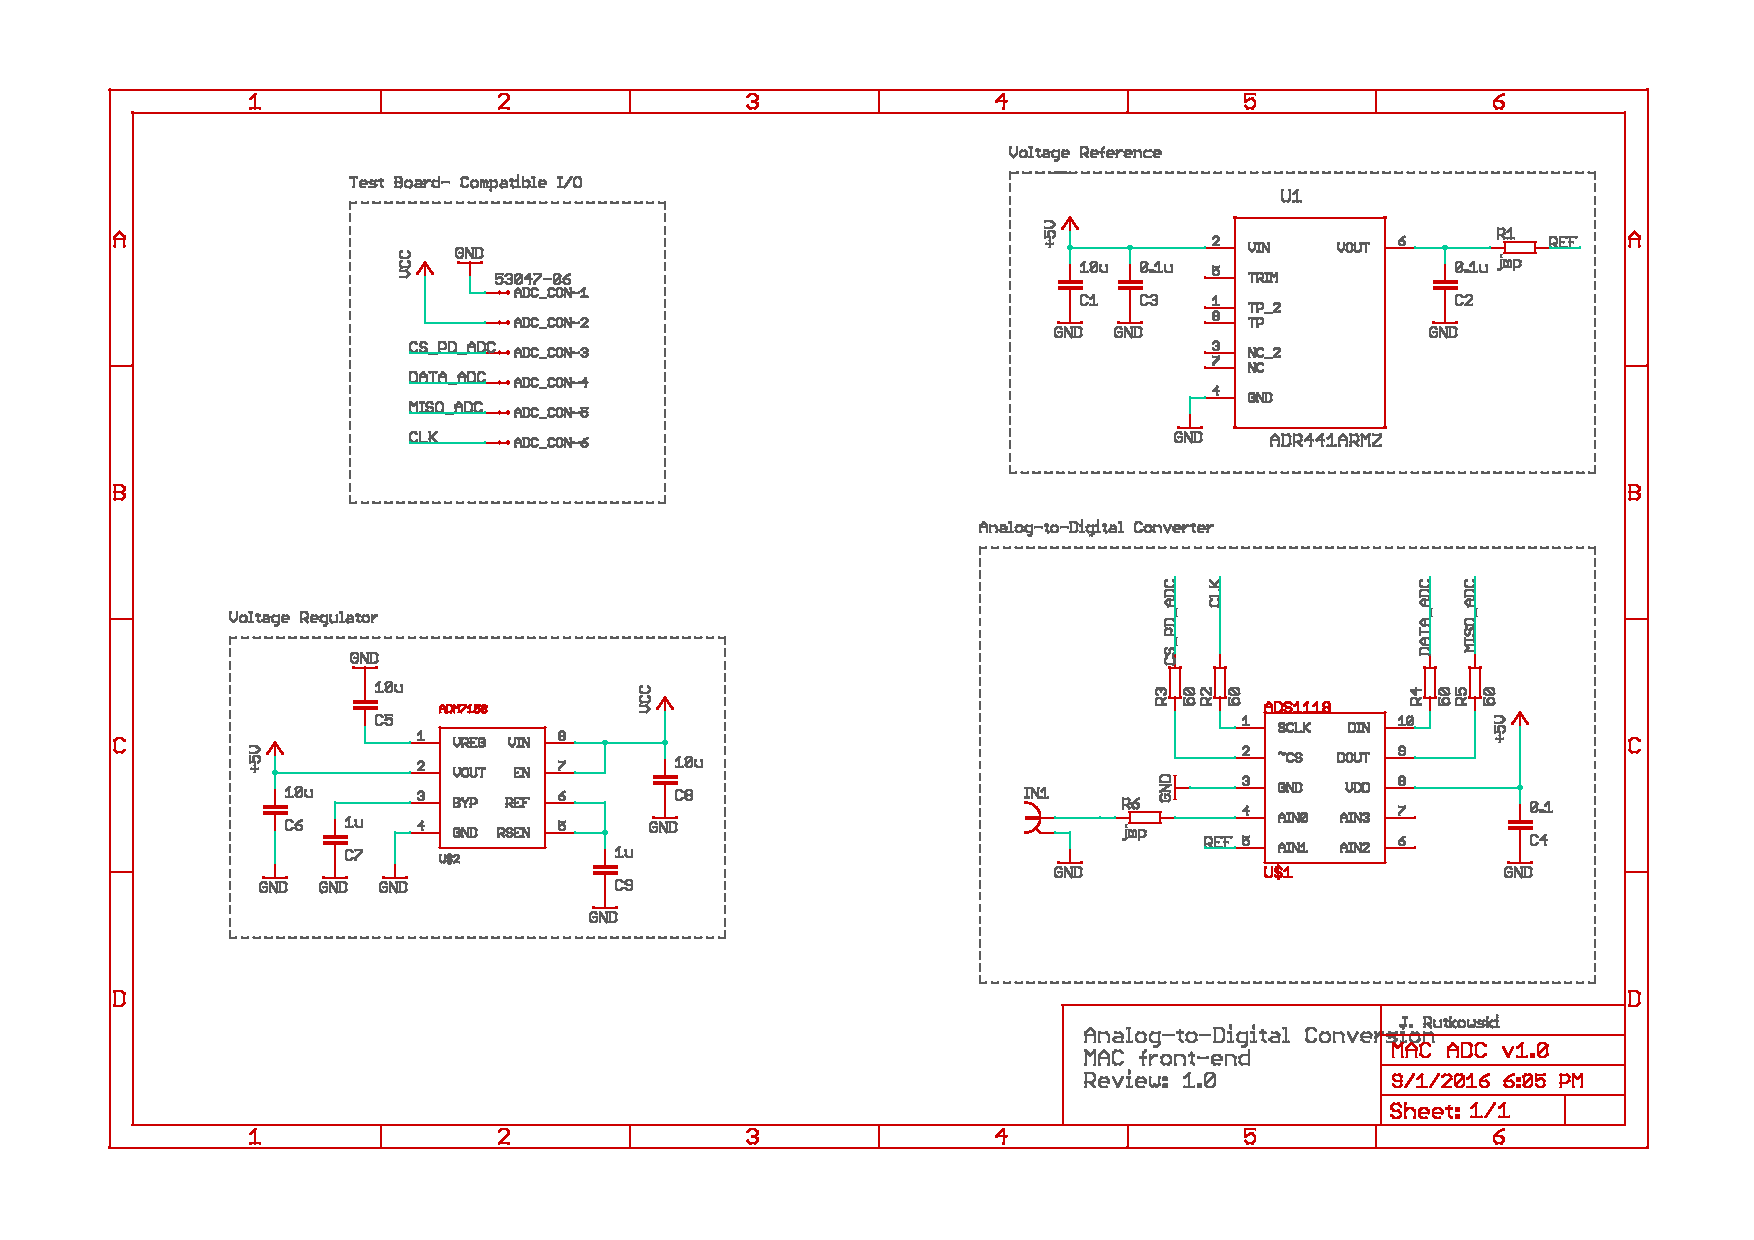
\includegraphics[width=\textwidth]{Images/MAC ADC v1.0.pdf}
    \captionsetup{justification=centering}
    \caption{ADC schematic.} 
    \label{fig:adc_sch}
\end{figure}

%equation
\begin{align}
\text{FSR} &= \pm 1.024\; V\nonumber\\
\text{Measure range}&=2.5 \pm \text{FSR} V\nonumber\\
\text{Measure range}&= 1.4760 \text{ V to } 3.5240 \text{ V}
\label{eq:full_range_1}
\end{align}

The LSb resolution\footnote{The LSb resolution represents the smallest interval that can be detected by the ADC.} was calculated to be $31.25 \;\mu \mathrm{V}$ (equation \ref{eq:lsb}).

\begin{align}
\text{LSb} &= \text{FSR}/2^{16} \nonumber\\
\text{LSb} &= \text{1.024}/2^{16} = 31.25 \;\mu \mathrm{V}
\label{eq:lsb}
\end{align}

In order to have a bigger measuring range, a compromise between FSR and LSb resolution must be made, as shown in table \ref{table:FSR}. To measure values from 0 to 5 V, the FSR of $\pm 4.096 \;\mathrm{V}$ must be selected. 

%table
\begin{table}[h!]
\centering
\begin{tabular}{|c|r|}
\hline
\textbf{FSR} & \textbf{LSb size} \\ \hline
$\pm$6.144 V     & 187.5 $\mu$V          \\ \hline
$\pm$4.096 V     & 125 $\mu$V            \\ \hline
$\pm$2.048 V     & 62.5 $\mu$V           \\ \hline
$\pm$1.024 V     & 31.25 $\mu$V          \\ \hline
$\pm$0.512 V     & 15.625 $\mu$V         \\ \hline
$\pm$0.256 V     & 7.8125 $\mu$V         \\ \hline
\end{tabular}
\caption{Full-scale range and corresponding LSb table.}
\label{table:FSR}
\end{table}
%Results of test (pending)
The new FSR function (listing \ref{lst:ADC_init_2}) was tested on \textit{Clock 1} and the results are presented in figure \ref{fig:adc_limitation_fixed}.

\begin{lstlisting}[style=c++,label={lst:ADC_init_2},caption={ADC\_startup() recommended function (file: mac.ino).},firstnumber=431,literate={mu}{$\mu$}1]
void ADC_startup() { // Starts ADS1118, FSR = 4.096 V
  SPI.setDataMode(SPI_MODE1);
  digitalWrite(CS_ADC, LOW);
  SPI.transfer(B00000010); // CR: ADC FSR = 4.096V, since Ref is 2.5 V, 
  SPI.transfer(B11100011); // CR: the measurement range is from -1.596 V to 6.596 V*
  digitalWrite(CS_ADC, HIGH); // CR: with a LSB size of 125 muV (LSB = FSR / 2^16).
  SPI.setDataMode(SPI_MODE0); // *Note: photodiode outputs never exceeds 6 V.
}
\end{lstlisting}

\begin{figure}[!h]
\centering
\begin{subfigure}[b]{0.49\textwidth}
	\centering
	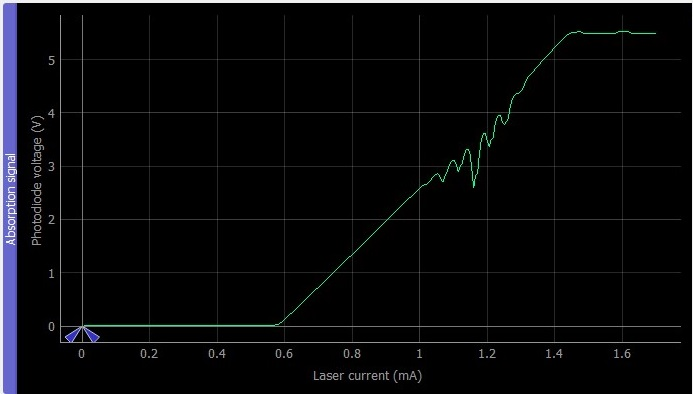
\includegraphics[height=0.6\textwidth]{Images/fsr_screenshot_after.jpg}
	\captionsetup{justification=centering}
\end{subfigure}
\hfill
\begin{subfigure}[b]{0.49\textwidth}
	\centering
	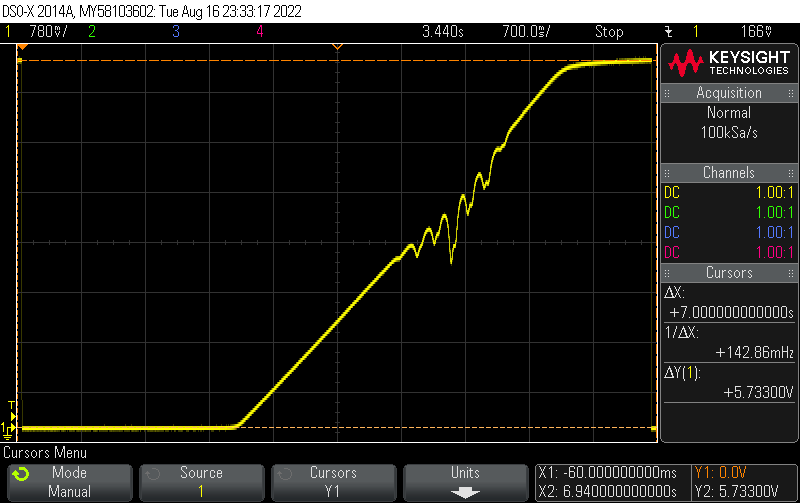
\includegraphics[height=0.6\textwidth]{Images/fsr_oscilloscope_after.jpg}
	\captionsetup{justification=centering}
\end{subfigure}
 \caption{Demonstrator's ADC limitation fixed.}
\label{fig:adc_limitation_fixed}
\end{figure}

After this modification it was necessary to recalculate the coefficients that allow the conversion from machine units to volts, the linear fit was computed with MATLAB from a new data set obtained from measuring the ADC value in machine units and its corresponding voltage value measured with the oscilloscope. The new coefficients and mathematical expression are found in equation \ref{eq:word_to_volt_1_2} and \ref{eq:word_to_volt_2_2}. The resulting fit presented in figure \ref{fig:word_to_volt_new} confirms the linear relation.

%Add equation and fit
\begin{align}
y=p1*x+p2\quad
\begin{cases}
p1=\SI{1.2448e-04}{}\\ p2=2.4863
\end{cases}
\label{eq:word_to_volt_1_2}
\\voltage=p1*ADC+p2 \quad\text{and}\quad ADC=\frac{(voltage-p2)}{p1}
\label{eq:word_to_volt_2_2}
\end{align}

\begin{figure}[!h]
    \centering
    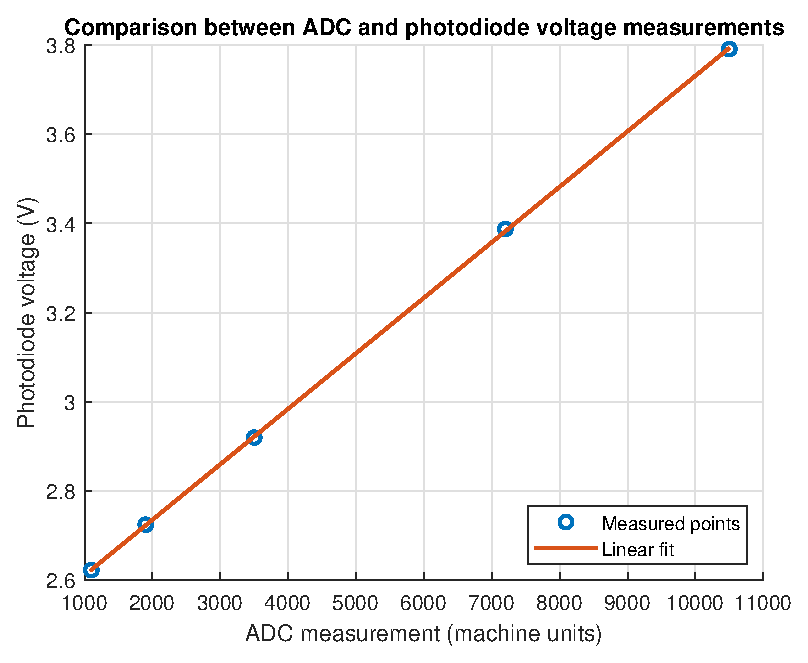
\includegraphics[width=0.6\textwidth]{Images/word_to_voltage_fsr_4.eps}
    \captionsetup{justification=centering}
    \caption{Improved linear fit between ADC and photodiode voltage measurements.} 
    \label{fig:word_to_volt_new}
\end{figure}

Finally, the new conversion functions are shown in listing \ref{lst:word_to_voltage_new}.
%Add listing

\begin{lstlisting}[style=python,label={lst:word_to_voltage_new},caption={Improved Python functions to convert machine units to voltage (file: misc.py).},firstnumber=151]
def word_to_voltage(value):
    #For FSR = 1.024 V
    # p1=0.000030294604198194861416565740186435
    # p2=2.4538899853718616483888581569772

    #For FSR = 4.096 V
    p1=0.00012448304623130003205427884793721
    p2=2.4863253857628526688472447858658
    return p1*value+p2
    
def voltage_to_word(value):
    #For FSR = 1.024 V
    # p1=0.000030294604198194861416565740186435
    # p2=2.4538899853718616483888581569772

    #For FSR = 4.096 V
    p1=0.00012448304623130003205427884793721
    p2=2.4863253857628526688472447858658
    return int((value-p2)/p1)
\end{lstlisting}

To confirm that the new reduced resolution did not affect the normal operation of the clocks, the \textit{Clock 1} was successfully locked on its CPT signal, as shown in figure \ref{fig:ADC_fix_check_CPT_lock}.

\begin{figure}[!h]
    \centering
    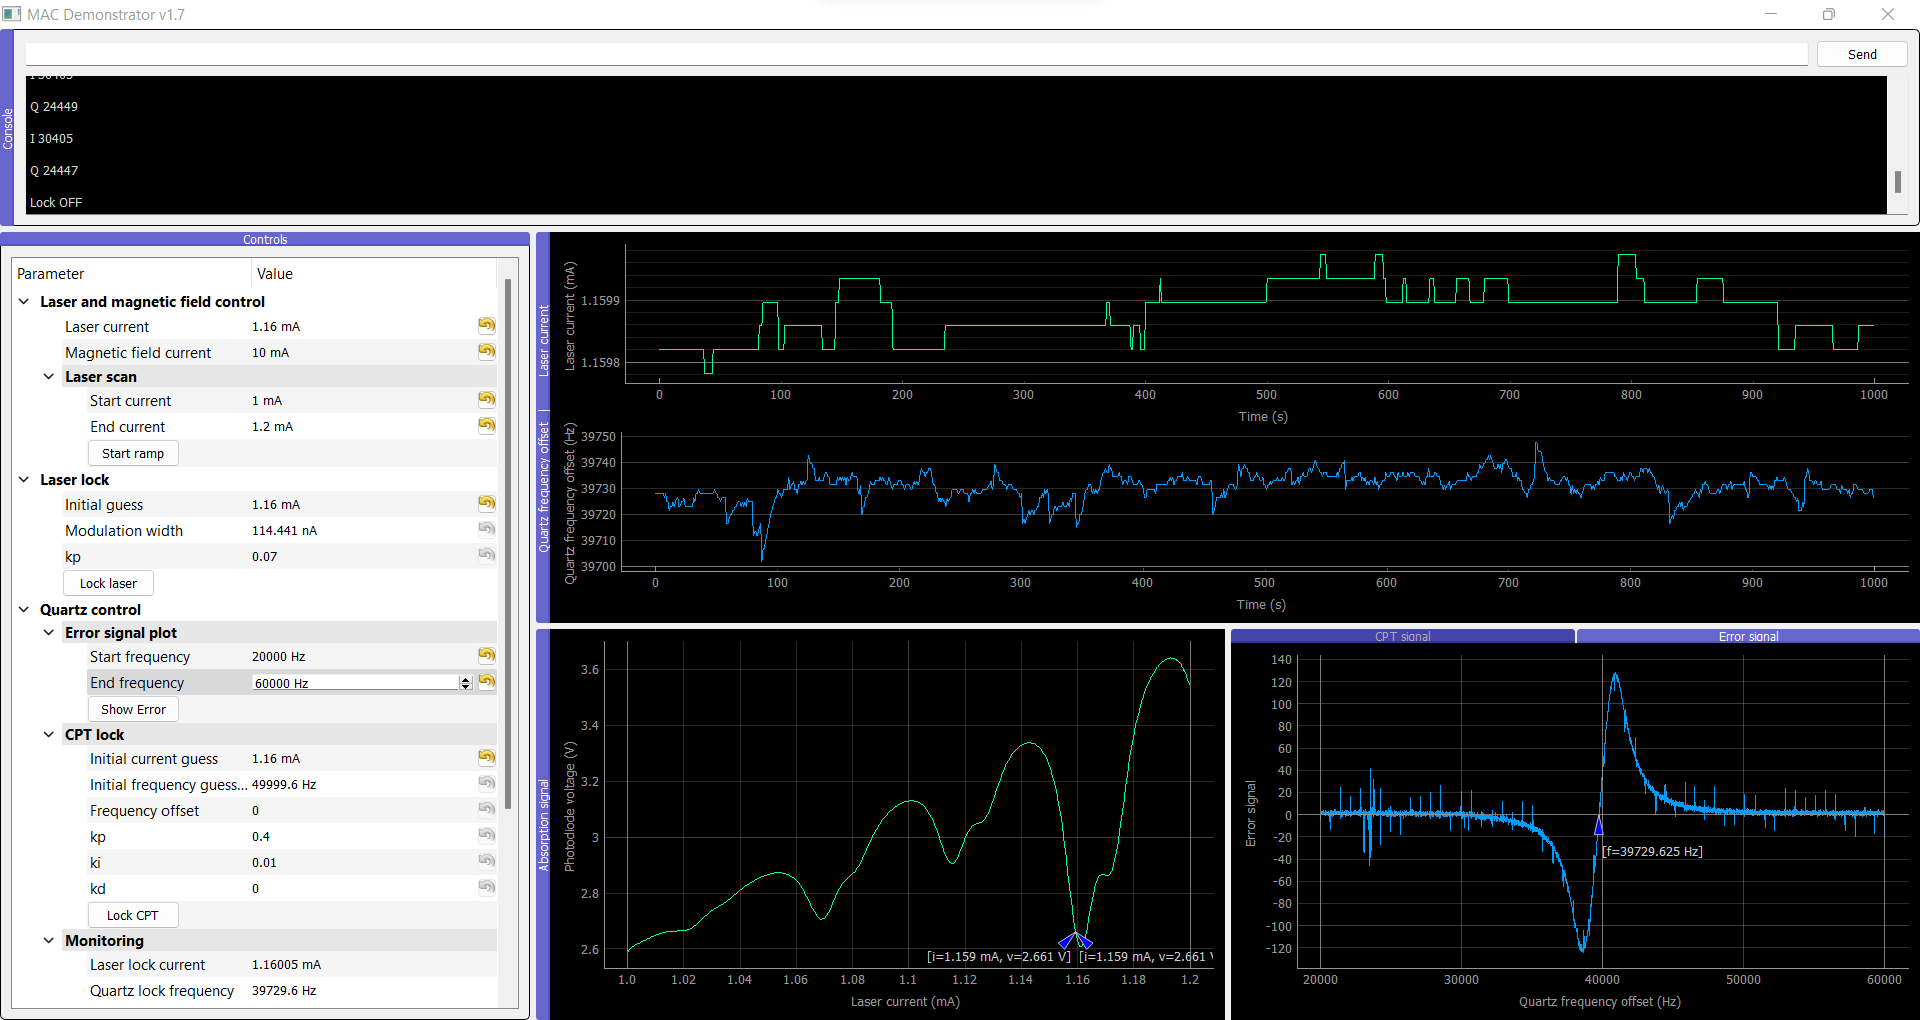
\includegraphics[width=\textwidth]{Images/CPT_lock_after_FSR_fix.png}
    \captionsetup{justification=centering}
    \caption{\textit{Clock 1} locked to its CPT signal after ADC limitation fixed.} 
    \label{fig:ADC_fix_check_CPT_lock}
\end{figure}

%
\newpage
\subsubsection{Addition of graph titles and axis labels}
\label{section:graphs}

All graphs were missing titles and axis labels, which resulted in a difficult to understand interface. In the new version, all the graphs are correctly labeled.

\subsubsection{Precise identification of maximum absorption}
\label{section:max_absorb}
 As shown in figure \ref{fig:plot_tools_1} a marker that indicates the minimum value found within the current measurement scope was implemented. This allows a precise identification of the laser current value at which the maximum absorption is found. 

\begin{figure}[!h]
\centering
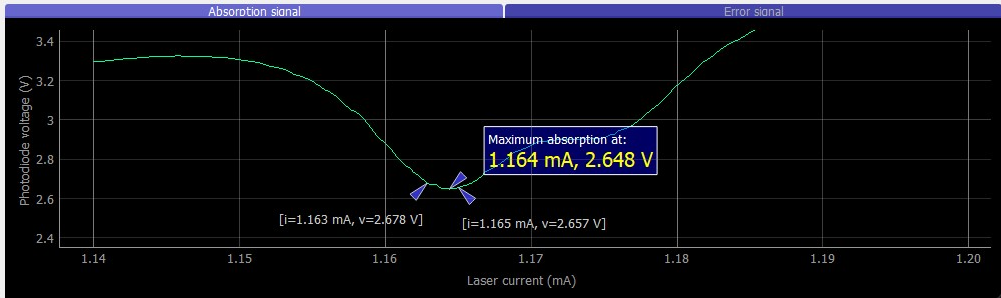
\includegraphics[width=\textwidth]{Images/plot_tools_1.png}
\captionsetup{justification=centering}
\caption{Plot tools for the absorption graph} 
\label{fig:plot_tools_1}
\end{figure}

\newpage    
\subsubsection{Graphical identification of locked/unlocked servo loops}
\label{section:lock/unlock}
%Explain lock and modulation

For didactic purposes, two separate arrow markers that highlight the current modulation measurement points were implemented in the "Absorption signal" graph (these markers become red if the lock state is lost and out of scope). The laser current value corresponding to the lock location is found at the middle of the modulation (figure \ref{fig:plot_tools_1}).

Similar to the previously described feature, it was desired to have a visual indicator of the quartz servo loop lock state (these markers become red if the lock state is lost and out of scope). As presented in figure \ref{fig:plot_tools_2}, now it's possible to visualize the locking offset frequency in both the CPT and Error signal graphs.
\begin{figure}[!h]
\centering
\begin{subfigure}[b]{0.49\textwidth}
\centering
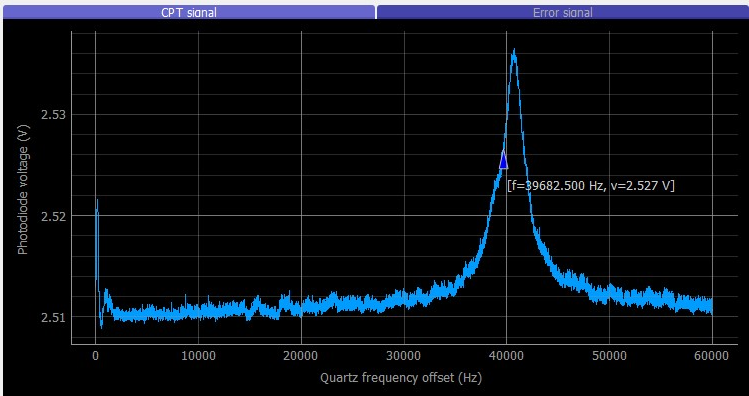
\includegraphics[height=0.52\textwidth]{Images/plot_tools_2.png}
\captionsetup{justification=centering}
\caption{CPT signal plot}
\label{fig:cpt_signal}
\end{subfigure}
\hfill
\begin{subfigure}[b]{0.49\textwidth}
\centering
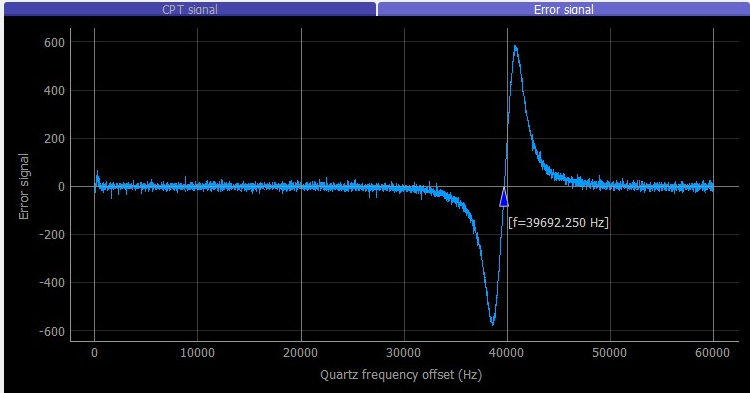
\includegraphics[height=0.52\textwidth]{Images/plot_tools_3.png}
\captionsetup{justification=centering}
\caption{Error signal plot}
\label{fig:error_signal}
\end{subfigure}
\caption{Plot tools for the CPT and Error signal} 
\label{fig:plot_tools_2}
\end{figure}
    
\subsubsection{Visualization of CPT signal}
\label{section:CPT}

In the original software, it was only possible to plot the error signal after a quartz scan (figure \ref{fig:error_signal}). We decided to also add the CPT transmission signal to the GUI for pedagogical purposes \mbox{(figure \ref{fig:cpt_signal})}.

\subsection{Measuring atomic clock stability}

To determine the stability of the atomic clock, we compute its Allan variance, which is a common way of characterizing the various sources of noise that can affect a clock stability. 

The instantaneous clock frequency $f_n$ is measured with an interval $\tau$, and we compute its mean value $<f>$. We then calculate the relative (or fractional) frequency $y_n = f_n / <f>$.
The Allan deviation is a measurement of the fractional frequency fluctuations for various integration times $\tau$.

The Allan variance for an integration time $\tau$ is given by:

\begin{equation}
\sigma^2 (\tau) = \frac{1}{2}* \langle (y_{n+1}-y_n)^2 \rangle
\end{equation}


%Consider the error measurements of a clock $x_n$, $x_{n+1}$, $x_{n+2}$ within interval $\tau$ \cite{allan1997science}. The normalized frequency departure average is 
% \begin{equation}
%     y_n = \frac{\Delta x_n}{\tau}
% \label{eq:average}
% \end{equation}
% The Allan variance is
% \begin{equation}
%     \sigma^{2} = \frac{1}{2\tau^{2}}(\Delta y^{2})
% \end{equation}
% Where $y$ is the normalized average frequency departure for the interval of $\tau$.
The Allan deviation is $\sigma$, the square root of the variance. The advantage of the Allan variance over standard variance is that the former can diverge for different types of noise independently of the number of samples. Another way to quantify the frequency instability is through the modified Allan deviation, which can differentiate between white noise and flicker PM noise. The purpose behind computing the Allan variance is that, ideally, the frequency spectrum is a straight line. However, due to noise, the frequency fluctuates between several values. The Allan variance quantifies how stable the frequency is through averaging the frequency over a certain average time. Practically, we select $\tau$ as an integration time and try to reconstruct the frequency signal by calculating the average. In this application, the instrument that we connected to measure the average and the Allan deviation is the Microsemi\slash Symmetricom 5120A, shown in figure \ref{fig:5125A}.

\begin{figure}[!h]
    \centering
    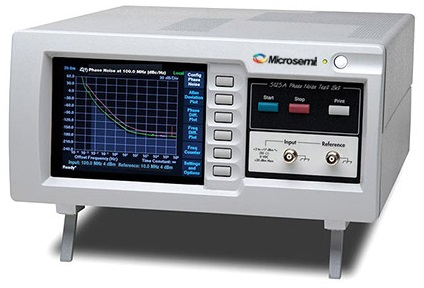
\includegraphics[width=0.5\textwidth]{Images/5125A.jpg}
    \captionsetup{justification=centering}
    \caption{Microsemi\slash Symmetricom instrument to measure Allan deviation} 
    \label{fig:5125A}
\end{figure}

We use figures \ref{fig:allan01}-\ref{fig:allan14} to illustrate Allan deviation measurements (the fractional frequency vs time data on the left were not taken for the CPT clocks, but this does not change the interpretation). \mbox{Figure \ref{fig:allan01}} corresponds to the smallest integration time, $\tau = 0.68\; s$. The fractional frequency fluctuations are $3x10^{-10}$. Figure \ref{fig:allan08} corresponds to an integration time of $86.8 s$ between each point. The relative frequency fluctuations are then much smaller, of about $2x10^{-11}$. Then finally, as shown in figure \ref{fig:allan14}, as $\tau$ increases, the Allan deviation is improved until a certain threshold where is reaches its minimum. After this threshold, increasing $\tau$ results in a frequency instability.

\begin{figure}[!h]
    \centering
    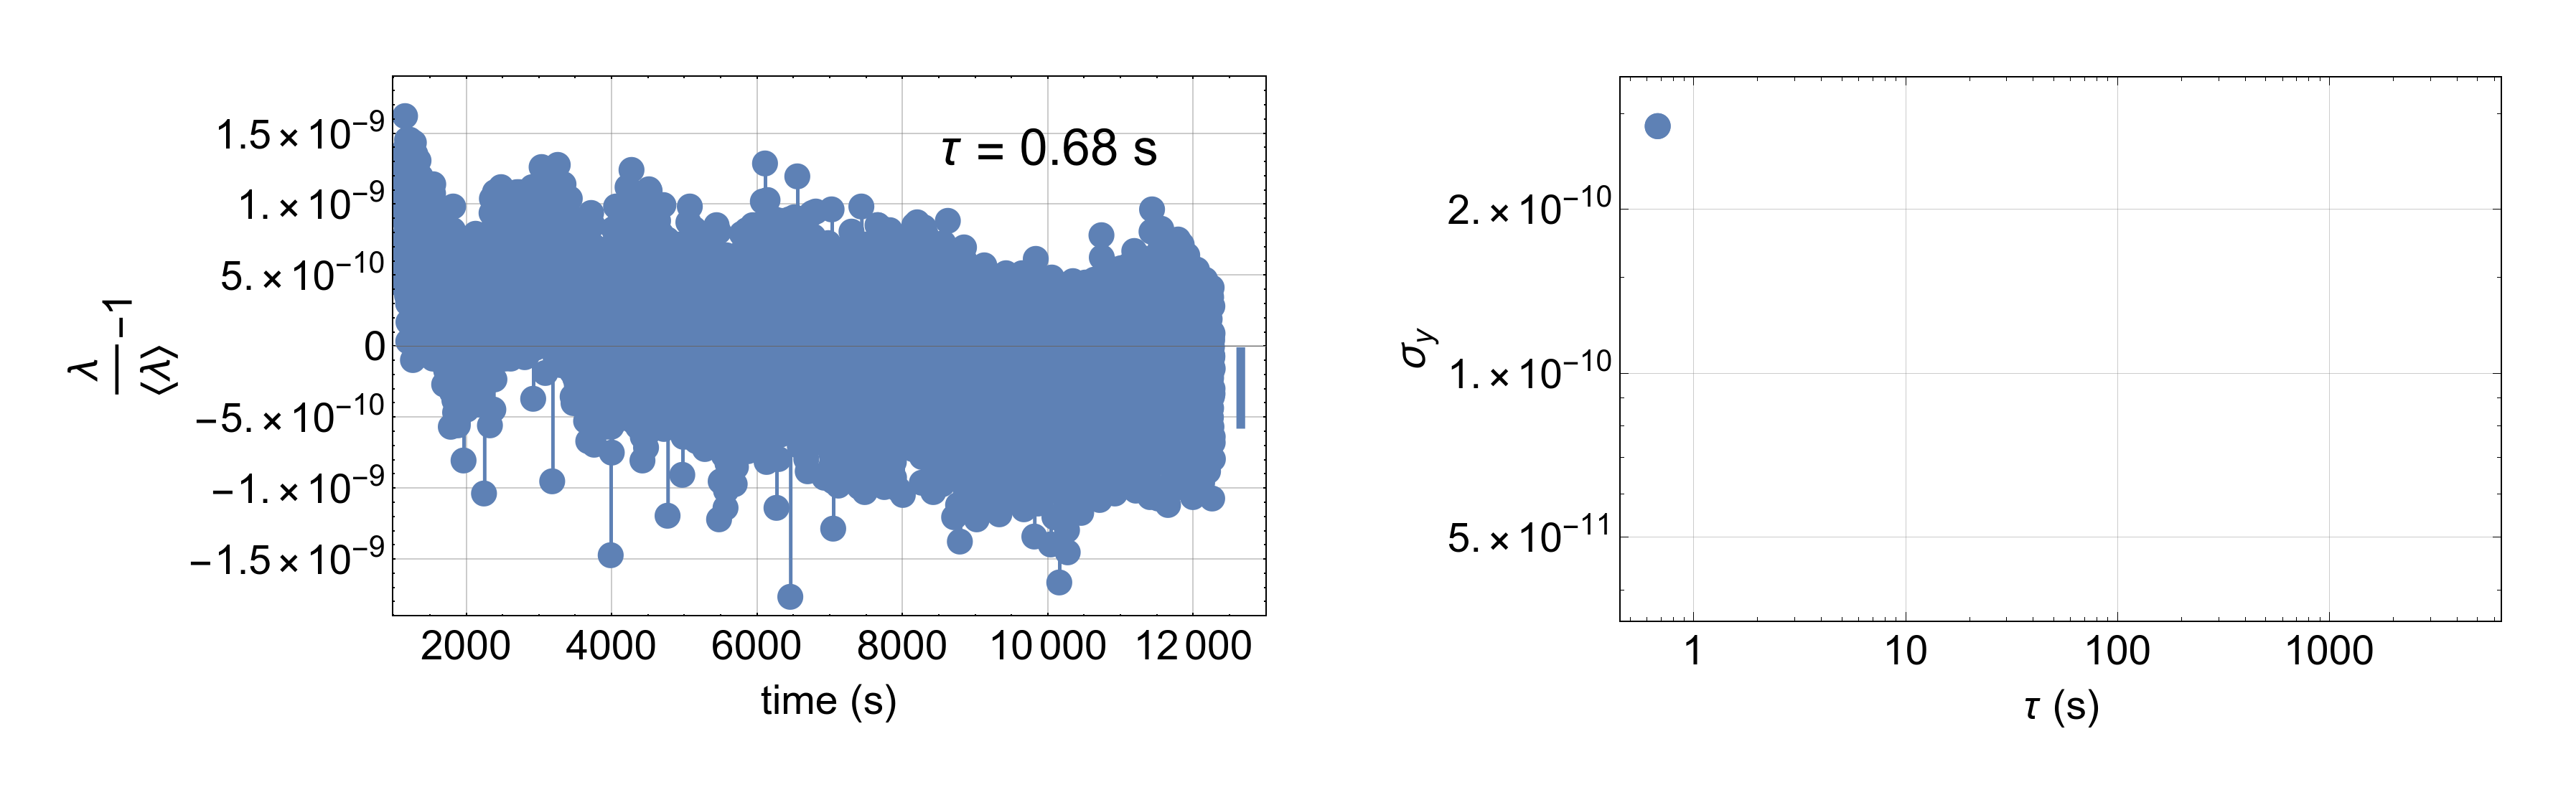
\includegraphics[width=0.9\textwidth]{Images/allan01.png}
    \captionsetup{justification=centering}
    \caption{Short term stability} 
    \label{fig:allan01}
\end{figure}
\begin{figure}[!h]
    \centering
    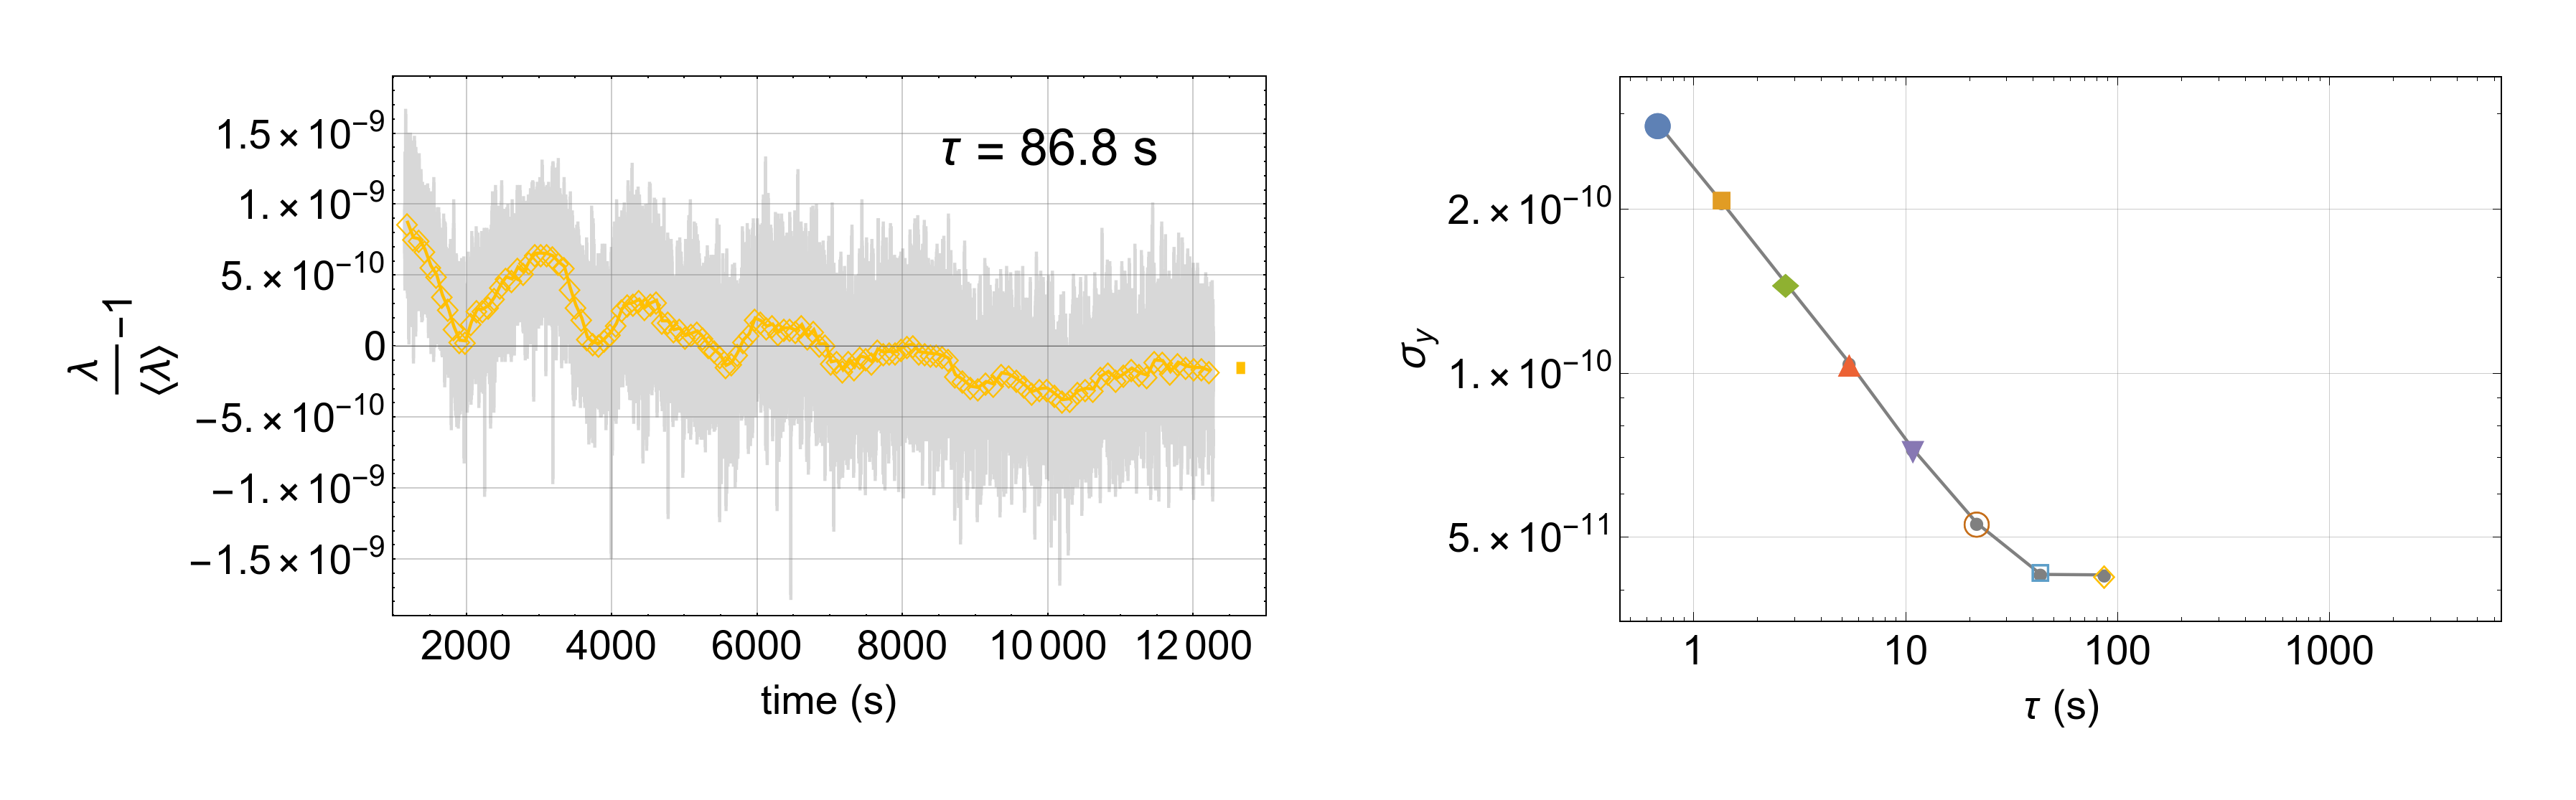
\includegraphics[width=0.9\textwidth]{Images/allan08.png}
    \captionsetup{justification=centering}
    \caption{Minimum Allan deviation threshold} 
    \label{fig:allan08}
\end{figure}
\begin{figure}[!h]
    \centering
    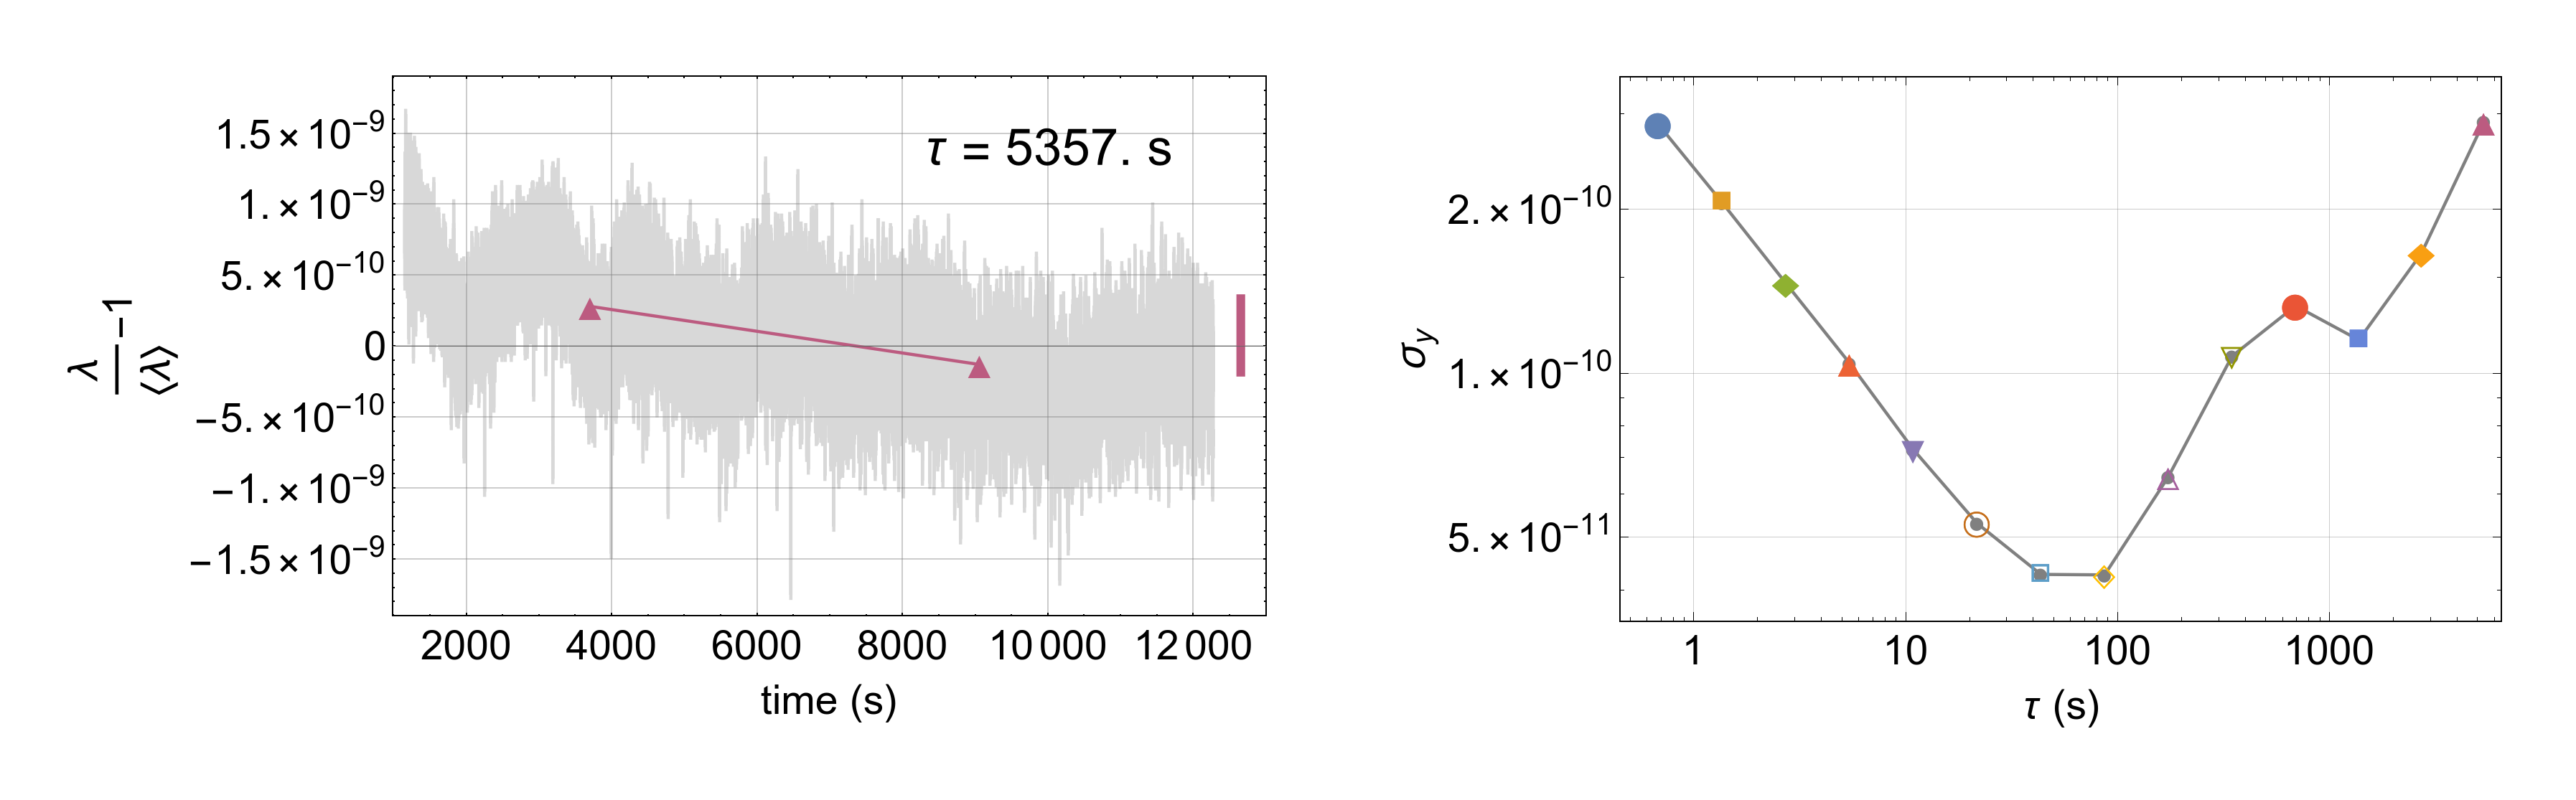
\includegraphics[width=0.9\textwidth]{Images/allan14.png}
    \captionsetup{justification=centering}
    \caption{Frequency instability} 
    \label{fig:allan14}
\end{figure}
\break
The Allan deviation of the free running quartz and quartz with locked servo loops was measured through the instrument. The values were extracted and plotted on MATLAB as shown in figure \ref{fig:stability_comp}. An important parameter when computing the Allan deviation is the average at 1 second, since it determines the short term stability. The free running quartz has a better short term stability than the one with locked servo loops. However, the latter is more stable with time, whereas the former loses the short term stability and becomes unstable after a certain period of time. The phase noise floor of the machine determines the threshold of the instrument sensitivity. In other words, measurements taken below the phase noise floor might not be as accurate.

\begin{figure}[!h]
    \centering
    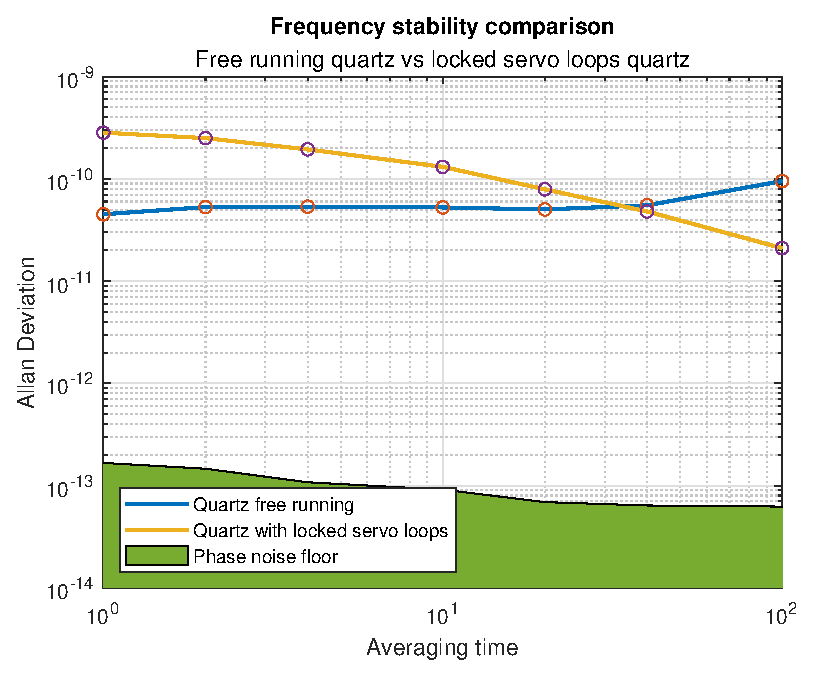
\includegraphics[width=0.7\textwidth]{Images/allan_deviation.eps}
    \captionsetup{justification=centering}
    \caption{Frequency stability comparison.} 
    \label{fig:stability_comp}
\end{figure}

% \subsection{Creation of documentation based on Arduino and Python code}
% \subsection{Implementation of unit tests for debugging purposes}

%Repair section:
\subsection{Repair of the two not working Atomic clocks}
\label{section:repair_atomic_clocks}

Two of the three atomic clock demonstrators were not operational, like \textit{Clock 2}, as shown in \mbox{figure \ref{fig:not_working_1}}. It could be identified a weak middle absorption, a very low signal-to-noise ratio, and both the "Error" and "CPT" signals were almost non-existent.

\begin{figure}[!h]
    \centering
    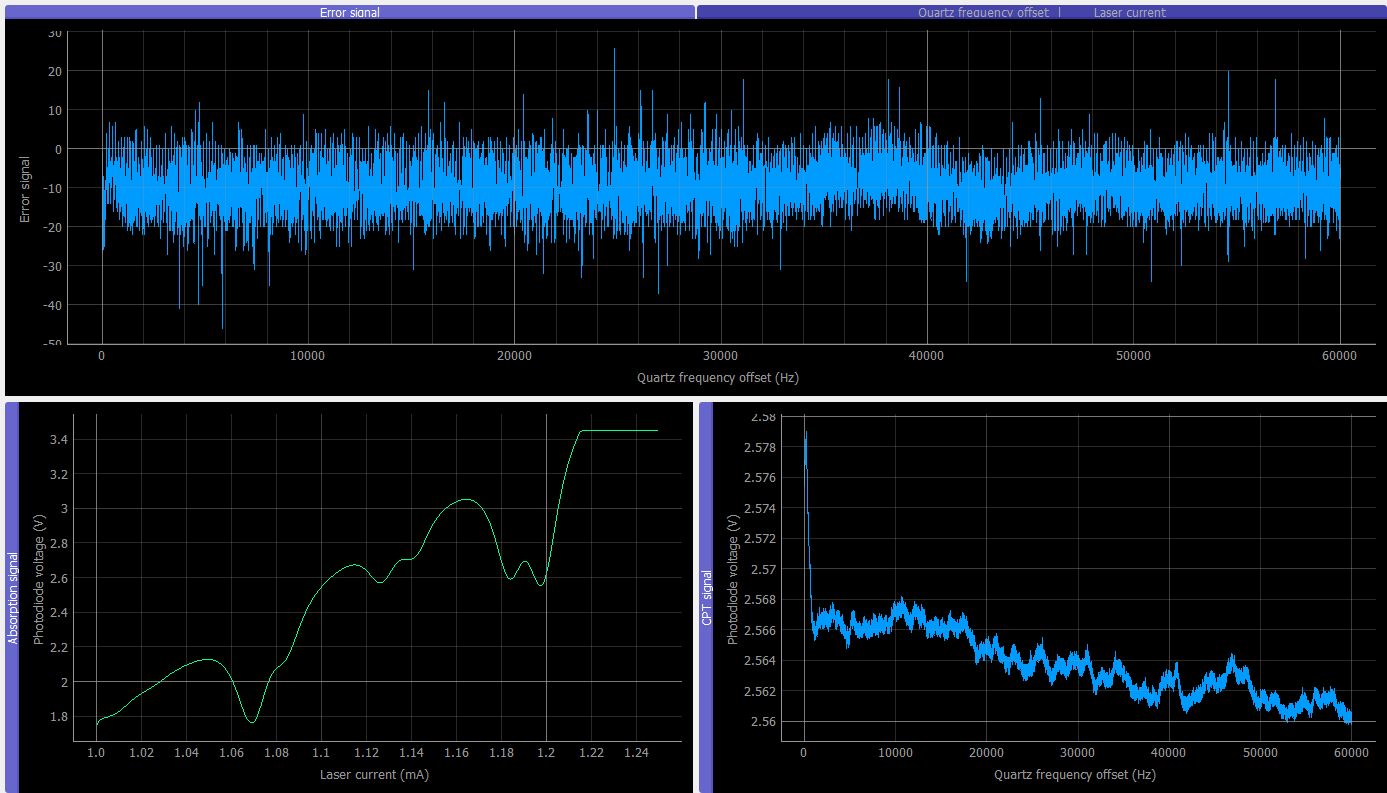
\includegraphics[width=0.5\textwidth]{Images/not_working.png}
    \captionsetup{justification=centering}
    \caption{\textit{Clock 2} not working properly.} 
    \label{fig:not_working_1}
\end{figure}

First, it was decided to test the Physical Packages of each clock (which is the combination of the Cs vapor cell, optics, laser, photodiode, heating element and magnetic field coil). The reason behind testing them is to determine if this was the root cause of the issue, considering that the three demonstrators were supposed to be identical.

As shown in figure \ref{fig:pp_test}, all the Physical Packages were working correctly when installed in the best working clock taken as reference (\textit{Clock 1}).

%PP1
\begin{figure}[!h]
\centering
\begin{subfigure}[b]{0.49\textwidth}
\centering
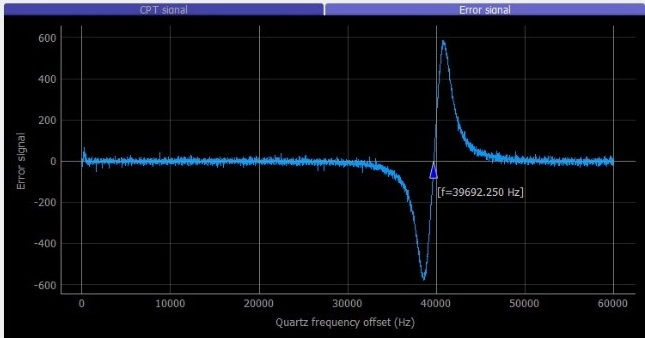
\includegraphics[height=0.5\textwidth]{Images/c1_pp1_1_2.jpg}
\captionsetup{justification=centering}
\caption{Error signal: Physical Package 1 in \textit{Clock 1}.}
\end{subfigure}
\hfill
\begin{subfigure}[b]{0.49\textwidth}
\centering
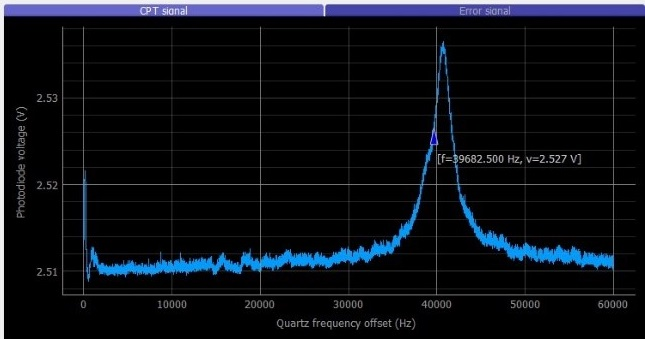
\includegraphics[height=0.5\textwidth]{Images/c1_pp1_2_2.jpg}
\captionsetup{justification=centering}
\caption{CPT signal: Physical Package 1 in \textit{Clock 1}.}
\end{subfigure}

%PP2
\centering
\begin{subfigure}[b]{0.49\textwidth}
\centering
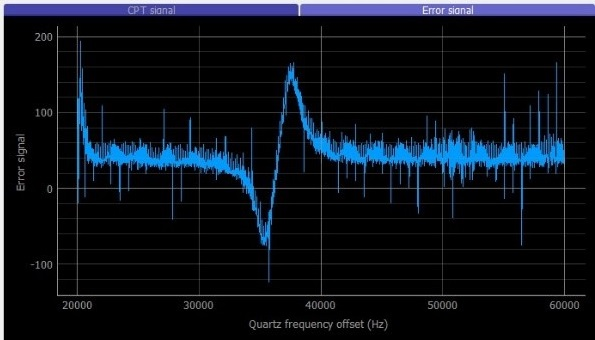
\includegraphics[height=0.5\textwidth]{Images/c1_pp2_1_2.jpg}
\captionsetup{justification=centering}
\caption{Error signal: Physical Package 2 in \textit{Clock 1}.}
\end{subfigure}
\hfill
\begin{subfigure}[b]{0.49\textwidth}
\centering
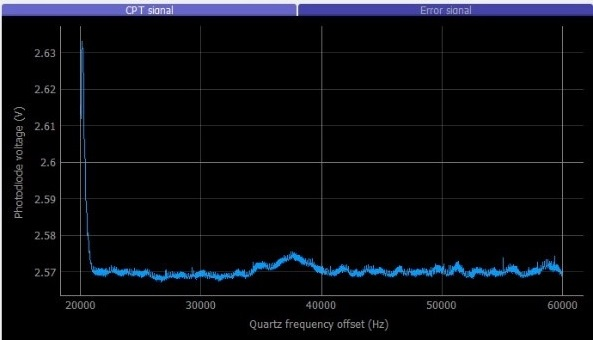
\includegraphics[height=0.5\textwidth]{Images/c1_pp2_2_2.jpg}
\captionsetup{justification=centering}
\caption{CPT signal: Physical Package 2 in \textit{Clock 1}.}
\end{subfigure}

%PP3
\centering
\begin{subfigure}[b]{0.49\textwidth}
\centering
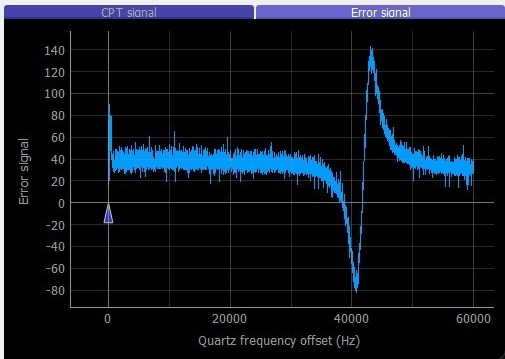
\includegraphics[height=0.52\textwidth]{Images/c1_pp3_1_2.jpg}
\captionsetup{justification=centering}
\caption{Error signal: Physical Package 3 in \textit{Clock 1.}}
\end{subfigure}
\hfill
\begin{subfigure}[b]{0.49\textwidth}
\centering
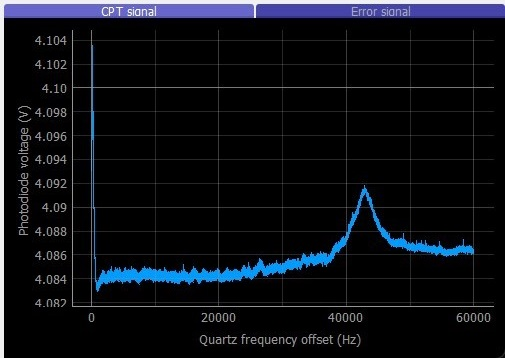
\includegraphics[height=0.52\textwidth]{Images/c1_pp3_2_2.jpg}
\captionsetup{justification=centering}
\caption{CPT signal: Physical Package 3 in \textit{Clock 1}.}
\end{subfigure}

\caption{Test of Physical packages in reference \textit{Clock 1}} 
\label{fig:pp_test}
\end{figure}

The next troubleshooting step was to test the microwave synthesizers in the best working clock (\textit{Clock 1}) to compare the results. As shown in figure \ref{fig:synth_test}, the synthesizer 1 and 2 have an incorrect "Error signal" and a very weak "CPT signal" which indicated an erratic modulation.

\begin{figure}[!h]
%PP2
\centering
\begin{subfigure}[b]{0.49\textwidth}
\centering
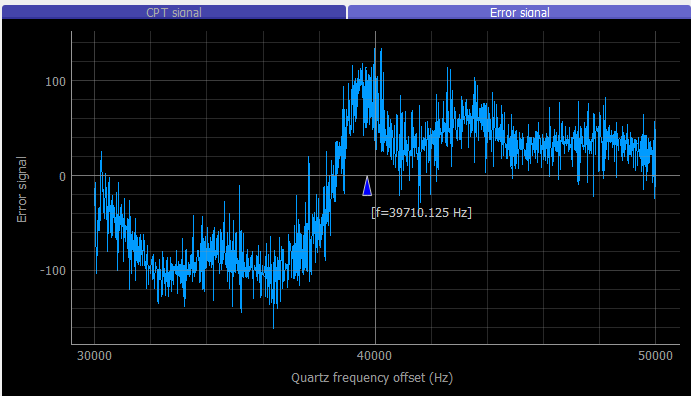
\includegraphics[height=0.5\textwidth]{Images/c1_synth_2_2_2.png}
\captionsetup{justification=centering}
\caption{Error signal: Synthesizer 2 in \textit{Clock 1}.}
\end{subfigure}
\hfill
\begin{subfigure}[b]{0.49\textwidth}
\centering
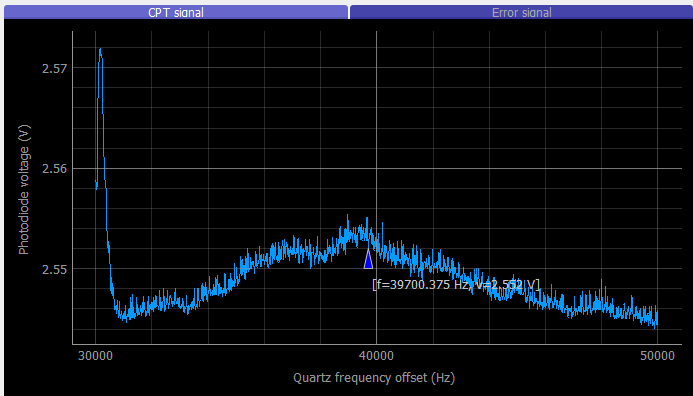
\includegraphics[height=0.5\textwidth]{Images/c1_synth_2_1_2.png}
\captionsetup{justification=centering}
\caption{CPT signal: Synthesizer 2 in \textit{Clock 1}.}
\end{subfigure}

%PP3
\centering
\begin{subfigure}[b]{0.49\textwidth}
\centering
\includegraphics[height=0.5\textwidth]{Images/c1_synth_3_2_2.png}
\captionsetup{justification=centering}
\caption{Error signal: Synthesizer 3 in \textit{Clock 1.}}
\end{subfigure}
\hfill
\begin{subfigure}[b]{0.49\textwidth}
\centering
\includegraphics[height=0.5\textwidth]{Images/c1_synth_3_1_2.png}
\captionsetup{justification=centering}
\caption{CPT signal: Synthesizer 3 in \textit{Clock 1}.}
\end{subfigure}

\caption{Test of Synthesizers in reference \textit{Clock 1}} 
\label{fig:synth_test}
\end{figure}

The synthesizer circuit consists of a ADF4158 fractional-N frequency synthesizer (maximum frequency at 6.1 GHz) with modulation and waveform generation capability; connected to a V950ME21-LF Voltage-Controlled Oscillator through a loop low filter, as shown in figure \ref{fig:sch_synth}. I found that the values of the components on the schematic were matching the ones on \textit{Clock 2} and \textit{Clock 3}, but were completely different for the \textit{Clock 1}. 

\begin{figure}[!h]
    \centering
    \includegraphics[width=0.7\textwidth]{Images/Frequency_synthesizer_v1.0.sch.pdf}
    \captionsetup{justification=centering}
    \caption{Circuit schematic of demonstrator's synthesizer before repair.} 
    \label{fig:sch_synth}
\end{figure}

Due to the discrepancy in the component values, the components of the synthesizer circuit of \mbox{\textit{Clock 1}} were desoldered to be measured, obtaining the values of table \ref{table:components}.

\begin{table}[!h]
\centering
\begin{tabular}{|c|c|c|}
\hline
\textbf{Components}    & \textbf{Clock 1}           & \textbf{Clock 2, 3 and Schematic} \\ \hline
\textbf{R1}  & $5.1\; \mathrm{k\Omega}$ & $147\; \mathrm{\Omega}$        \\ \hline
\textbf{R2}  & $2.4\; \mathrm{k\Omega}$ & $83\; \mathrm{\Omega}$         \\ \hline
\textbf{R3}  & $4.7\; \mathrm{k\Omega}$ & $5.1 \mathrm{k\; \Omega}$      \\ \hline
\textbf{C14} & $330\; \mathrm{pF}$                     & $47\; \mathrm{nF}$                            \\ \hline
\textbf{C15} & $8.2\; \mathrm{nF}$                     & $680\; \mathrm{nF}$                           \\ \hline
\textbf{C16} & $680\; \mathrm{pF}$                     & $22\; \mathrm{nF}$                            \\ \hline
\end{tabular}
\caption{Loop filter components.}
\label{table:components}
\end{table}

After simulating the time and frequency domain behavior of the circuit in ADIsimPLL software (figure \ref{fig:simulation_1}), it was found that the loop bandwidth of the filter in \textit{Clock 2} and \textit{Clock 3} was 4.81 kHz, whereas, for the \textit{Clock 1} was 61.6 kHz. 

\begin{figure}[!h]
\centering
\begin{subfigure}[b]{\textwidth}
\centering
\includegraphics[width=0.8\textwidth]{Images/freq_simu_1.jpg}
\captionsetup{justification=centering}
\caption{Phase Noise simulation of synthesizer loop filter \textit{Clock 2 and 3}.}
\end{subfigure}
\newline
\begin{subfigure}[b]{\textwidth}
\centering
\includegraphics[width=0.8\textwidth]{Images/freq_simu_2.jpg}
\captionsetup{justification=centering}
\caption{Phase Noise simulation of synthesizer loop filter \textit{Clock 1}.}
\end{subfigure}
\caption{Comparison between synthesizer's Phase Noise simulation.} 
\label{fig:simulation_1}
\end{figure}

The loop bandwidth determines the frequency and phase lock time, lower values of loop bandwidth lead to reduced levels of phase noise and reference spurs, but at the expense of longer lock times and less phase margin.\cite{pll}

Indeed, the Time Domain simulation shows a lock time of approximately 1.5 ms for the \textit{Clock 2} and \textit{Clock 3}; and $25\; \mathrm{\mu s}$ for the \textit{Clock 1} (figure \ref{fig:time_simu}). 

\begin{figure}[!h]
\centering
\begin{subfigure}[b]{0.49\textwidth}
\centering
\includegraphics[width=\textwidth]{Images/time_simu_1.jpg}
\captionsetup{justification=centering}
\caption{Lock Time simulation of synthesizer loop filter \textit{Clock 2 and 3}.}
\end{subfigure}
\hfill
\begin{subfigure}[b]{0.49\textwidth}
\centering
\includegraphics[width=\textwidth]{Images/time_simu_2.jpg}
\captionsetup{justification=centering}
\caption{Lock Time simulation of synthesizer loop filter \textit{Clock 1}.}
\end{subfigure}
\caption{Comparison between synthesizer's Lock Time simulation.} 
\label{fig:time_simu}
\end{figure}

By replacing the components to match those of \textit{Clock 1} (figure\ref{fig:components_replacement}) it is now possible to have a 60 times faster lock time with a 12 times wider loop bandwidth.

\begin{figure}[!h]
    \centering
    \includegraphics[width=0.9\textwidth]{Images/Synthesizer 1 - Components}
    \captionsetup{justification=centering}
    \caption{Replaced components based on \textit{Clock 1}.} 
    \label{fig:components_replacement}
\end{figure}

Finally, the components were replaced on synthesizer 2 and 3 and the circuits were tested on \mbox{\textit{Clock 1}} (as shown in figure \ref{fig:synth_final}), this solved the problem and now the three Atomic Clocks are operational and able to lock on the CPT transition.

\begin{figure}[!h]
\centering
\begin{subfigure}[b]{0.49\textwidth}
\centering
\includegraphics[width=\textwidth]{Images/synth_2_before.png}
\captionsetup{justification=centering}
\caption{Synthesizer 2 - before.}
\end{subfigure}
\hfill
\begin{subfigure}[b]{0.49\textwidth}
\centering
\includegraphics[width=\textwidth]{Images/synth_2_after.png}
\captionsetup{justification=centering}
\caption{Synthesizer 2 - after.}
\end{subfigure}
\newline
\centering
\begin{subfigure}[b]{0.49\textwidth}
\centering
\includegraphics[width=\textwidth]{Images/synth_3_before.png}
\captionsetup{justification=centering}
\caption{Synthesizer 3 - before.}
\end{subfigure}
\hfill
\begin{subfigure}[b]{0.49\textwidth}
\centering
\includegraphics[width=\textwidth]{Images/synth_3_after.png}
\captionsetup{justification=centering}
\caption{Synthesizer 3 - after.}
\end{subfigure}
\caption{Synthesizers 2 and 3 on \textit{Clock 1} before and after components replacement.} 
\label{fig:synth_final}
\end{figure}

\subsection{Recommendations}
It is worth pointing out the following recommendations for the clocks operation, as well as possible improvements that can be made to future versions of the software and hardware:

\begin{itemize}
    \item The best results in terms of stability were found when the middle absorption profile containing the CPT signal was positioned at 2.5 V or 2.6 V (by controlling the VCSEL temperature externally), since this is the middle of the ADC's measuring range.
    \item I recommend the ground terminal of the AC connector to be linked to the GND plane of the circuits, as this was found to be a considerable source of noise in the signal, specially when no instruments are connected to the demonstrator.
    \item I recommend the vapor cell of \textit{Clock 2} is replaced since the absorption signal was very weak, this leads to problems in locking both the laser and the quartz frequency. Furthermore, even though \textit{Clock 2} is now operational, it appears that the elements on the microwave section are disturbing and attenuating the signal.
    \item The larger the laser current scan range, the slower the refresh rate for the absorption graph becomes. This is due to the fact that a delay was added in the microcontroller code to make sure that the signal has the same period on the oscilloscope whether the data is being transmitted to the computer or not. To solve this limitation, and since the oscilloscope is no longer required, the delay can be removed on Arduino code (file: mac.ino, line: 686) for a faster response.
\end{itemize}

\subsection{Partial conclusion}
The improvements done in the CPT-based Cs microcell Atomic Clock pedagogical model are related to several aspects, like including a more intuitive and capable graphical user interface. For example, the controls are no longer in terms of machine units but in the respective physical unit. Also, there are now visual tools to have a precise value of the maximum absorption point and the locking current and frequency. Additionally, I was able to fix two of the Atomic Clocks that were not working properly by analyzing and modifying their Phase lock loop synthesizer circuits. The improvements added to this project are very significant compared to the previous version. 
\section{Final conclusion}
The two projects that are part of my Master 1 internship are the "Superradiant laser instrumentation process" and "Improvements on CPT-based Cs microcell Atomic Clock
pedagogical model". The former project included the implementation of a robust communication protocol between the instrumentation elements in the laboratory, that was previously erratic. Also, another significant contribution for this project was the addition of a standalone single board computer (LattePanda) to run the wavelength meter software and UDP server written in C++. 

As for the second project, it is related to the atomic clock used in yearly EFTS, which required plenty of improvements to work in a satisfactory and reliable manner. This will allow the attendees of EFTS to have the opportunity to focus on the theory behind the atomic clock, instead of focusing too much on how to control the elements in a non-intuitive manner. %As future improvements, the ground from the outlet should be connected to the atomic clock circuit ground. This would solve the problem of having a high level of noise when no instruments are connected. And also the Atomic \textit{Clock 2} signal can be improved, even though it's now operational, it appears that the elements on the microwave section are disturbing and attenuating the signal.
%References:
\section{Acknowledgment}
I gratefully thank Dr. Marion DELEHAYE, Dr. Rodolphe BOUDOT and Dr. Jean-Michel FRIEDT for their help and time to guide me in both projects.
% \newpage
\bibliographystyle{unsrt} % We choose the "plain" reference style
\bibliography{refs} % Entries are in the refs.bib file

\end{document}